

% !TeX encoding = UTF-8
% !TeX spellcheck = fr_FR
% !TeX root = ../mythesis.tex
% !TeX program = pdflatex (build)
%%% TeXmaker : no 'magic comments' but set Root with Options > Set as master file

%useful stuff for what follows
\newcommand{\xbf}{\pmb{x}}
\newcommand{\ci}{\mathrm{i}}
\newcommand{\ee}{\mathrm{e}}
\newcommand{\lr}[1]{\left(#1\right)}
\newcommand{\lrsq}[1]{\left[#1\right]}
\newcommand{\tp}{\mathrm{p}}
\newcommand{\tv}{\mathrm{v}}
\newcommand{\vtv}{\boldsymbol{\mathrm{v}}}
\newcommand{\vna}{\boldsymbol{\nabla}}
\newcommand{\vx}{\mathbf{x}}
\newcommand{\tx}{\mathrm{x}}
\newcommand{\vobf}{\pmb{v_0}}
\newtheorem{theorem}{Theorem}
\newtheorem{lemma}[theorem]{Lemma}

\newcommand{\kbf}{\mathbf{k}}
\newcommand{\vbf}{\pmb{v}}
\newcommand{\rbf}{\mathbf{r}}
\newcommand{\ombog}{\omega_{\mathrm{b}}}
\newcommand{\betin}{\beta^{\mathrm{in}}}
\newcommand{\betout}{\beta^{\mathrm{out}}}
\newcommand{\rmexp}{\mathrm{exp}}
\newcommand{\im}{\mathfrak{Im}}
\newcommand{\re}{\mathfrak{Re}}
\newcommand{\mbogo}{m_{\mathrm{det}}}
\newcommand{\cs}{c_{\mathrm{s}}}
\newcommand{\dpsi}{\delta\psi}
\newcommand{\opsi}{\hat{\psi}}
\newcommand{\odpsi}{\hat{\delta\psi}}
% \newcommand{\norm}[1]{\left\lVert#1\right\rVert}
\newcommand{\dr}{\mathrm{d}\mathbf{r}}
\newcommand{\Lbog}{\mathcal{L}_B}
\newcommand{\ha}{\hat{a}}
\newcommand{\hadag}{\hat{a}^\dagger}
\newcommand{\hb}{\hat{b}}
\newcommand{\hbdag}{\hat{b}^\dagger}

\setcounter{topnumber}{2}
\setcounter{bottomnumber}{0}
\setcounter{totalnumber}{2}
\renewcommand{\topfraction}{0.99}
\renewcommand{\textfraction}{0.01}
\renewcommand{\floatpagefraction}{0.8}


\graphicspath{{./}{./fig/}{./chap_Ag_theory/fig/}}

\chapter{Hawking radiation in a polariton quantum fluid}
\label{chap:AG_theory}

After introducing the polariton system that will be used for quantum simulations, we present the theoretical framework that  
describes Hawking radiation in a polariton quantum fluid. In this chapter, we will first establish the original hydrodynamical analogy between the propagation 
of acoustic waves in a moving fluid and scalar fields in curved spacetime. This analogy is at the heart of what motivated the study 
of Hawking radiation in analog systems, leading to a first generation of experiment in classical systems such as water tanks. These experiments
\cite{rousseaux_observation_2008,weinfurtner_measurement_2011} demonstrated positive to negative frequency conversion of shallow surface waves in the vicinity of a sonic horizon. However the temperature
of classical fluids is too high to observe quantum effects. More precisely, Hawking radiation is expected to create entanglement between the emitted modes which can not be tested with water waves. 
Quantum fluids appear then as promising candidate since the 
fluctuations around the ground or steady state require a quantum treatment to be understood. In fact we will see that describing a fluid with trans-critical flow in the framework of the Bogoliubov theory also predicts particle creation from vacuum. Studying the effect from this point of view will reveal a strong robustness 
of the effect beyond the original hydrodynamical approach and widen the range of regimes where Hawking radiation can be observed.


\section{The hydrodynamical analogy}

In the previous chapter, we established that the dynamics of microcavity polaritons can be described by a driven dissipative Gross-Pitaevskii equation.
By writing the wavefunction in terms of phase and density, this equation can be cast into a continuity equation and an Euler equation for a non-barotropic fluid in the pump rotating frame. Starting from the GPE,
a polariton system resonantly pumped by a laser of the general form $F_{\tp}e^{i\phi(x,t)}$ leads the fluid to a state described by the wavefunction $\psi(x,t)=\sqrt{n_0}e^{i\phi(x,t)}$. The phase and modulus $\psi$ :
\begin{equation}
    \begin{align}
    \partial_t \phi +& \frac{\mlp v_0^2}{2\hbar}+\frac{\hbar}{2\mlp}\frac{\partial_x^2\sqrt{n_0}}{\sqrt{n_0}}+V_{LP}+gn+g_rn_r+\frac{\re\lrsq{F_{\tp}e^{-i\theta}}}{\mlp}=0\,\\
    \partial_t n_0 +& \partial_x(n_0v)= \gamma n_0 -2\im\lrsq{F_{\tp}e^{-i\theta}}\sqrt{n_0}
    \end{align}
    \label{eq:continuity}
\end{equation}
If we neglect the drive and dissipation terms which is the situation of a conservative fluid, we recover the original equation describing 
sound waves in a moving flow. This is precisely the equation that was used in the initial analogy made by W. Unruh \cite{unruh_experimental_1981}.
However, the out of equilibrium nature of the microcavity polaritons brings different phenomenology. In particular, perturbations propagating in
the fluid are not necessary sound waves as we will se later. It means that the dispersion of these perturbations is not linear and 
can remarkably exhibit a gap which can be associated to massive excitations. To avoid making approximations it is convenient to make the same calculations in the pump rotating frame. It equivalently means that all frequencies
will be taken with respect to the pump. In practice this is done by writing the pump $F_{\tp}(x)= F_{\tp}e^{i\theta_p(x)}$ with $\theta_p(x)=k_px$ and looking for steady state wavefunction 
of the same form $\psi(x,t)=\sqrt{n_0}e^{i\theta_p(x)}$. Plugging this into the GPE we obtain that the phase and density of the fluid must fulfill the following equation :

\begin{equation}
    \lrsq{-\frac{\hbar}{2\mlp}\nabla^2-i\frac{\hbar}{2}(\vna\cdot\pmb{v_0}) -i\hbar(\pmb{v_0}\cdot\vna)- \delta(v_0)+g_{\rm r}n_{\rm r}+g n_0-\ci\frac{\hbar\gamma}{2}}\sqrt{n_0}+|F_\tp|=0\,
        \label{eq:StatHomogEOSDens}
\end{equation}
with $\hbar \delta(v_0)=\hbar\omega_\tp-\hbar\omega_0-\mlp v_0^2/2$ (note that this is just $\delta(k_p)$ in a homogeneous configuration where $\pmb{v_0}=\hbar\pmb{k_p}/\mlp$).
To study the low energy collective perturbations of the fluid state we linearize the system around the steady state by writing the wavefunction
$\psi(x,t)=(\sqrt{n_0}+e^{-\gamma t/2}\delta\psi(x))e^{i\theta_p(x)}$ where the term $e^{-\gamma t/2}$ account for the losses as we will see later. Injecting this expression in \autoref{reservoir_eq} and using \autoref{eq:StatHomogEOSDens} we obtain to linear order in $\delta\psi$ :

\begin{equation}
    \ci \hbar \lr{\partial_t+\pmb{v_0}\cdot{\vna}}\delta\psi=\lrsq{-\frac{\hbar}{2\mlp}\nabla^2+\rho-\ci\sigma}\delta \psi+g n_0 \delta\psi^*,
        \label{eq:DefPertGPE}
\end{equation}
where $$\rho\coloneqq2g n_0- \delta(v_0)+g_{\rm r}n_{\rm r}\qquad\text{and}\qquad\sigma\coloneqq\hbar/2\vna \cdot\pmb{v_0}.$$
The term $\sigma$ encodes the gradient of the fluid velocity field and is zero for a homogeneous velocity background. 
Note that here we have assumed that there is no external potential without loss of generality since it can be included in the definition of $\rho$.

\bigskip

The above equation and its complex conjugate can be seen as a system of two coupled partial differential equations (PDEs) of first order in time-derivatives and second order in space-derivatives. A way to solve this system is by rewriting it as a single PDE of second order in time and fourth order in space. To that end, we solve $\delta \psi^*$ in terms of $\delta \psi$ from the above equation to obtain
\begin{equation}
    \delta \psi^*=\frac{1}{g n_0}\lrsq{\ci \hbar (\partial_t+\pmb{v_0}\cdot{\vna})+\frac{\hbar}{2\mlp}\nabla^2-\rho+\ci\sigma}\delta \psi.
    \label{eq:hydropsi_conj}
\end{equation}
Plugging this into the complex conjugate equation of \eqref{eq:DefPertGPE} we find
\begin{equation}
\begin{split}
    \ci \hbar &\lr{\partial_t+\pmb{v_0}\cdot{\vna}}\frac{1}{g n_0}\lrsq{\ci \hbar \lr{\partial_t+\pmb{v_0}\cdot{\vna}}+\frac{\hbar}{2\mlp}\nabla^2-\rho+\ci\sigma}\delta \psi=\\
    %%%%%%
    &\lrsq{\lr{\frac{\hbar}{2\mlp}\nabla^2-\rho-\ci\sigma}\frac{1}{g n_0}\lr{\ci \hbar \lr{\partial_t+\pmb{v_0}\cdot{\vna}}+\frac{\hbar}{2\mlp}\nabla^2-\rho+\ci\sigma}-g n_0} \delta \psi
\end{split}
    \label{eq:SecOrdPhi}
\end{equation}
For homogeneous backgrounds we have $\sigma=0$ and $\delta(v_0)=\delta(k_{\tp})$. Hence, the above equation \eqref{eq:SecOrdPhi} can be simplified to
\begin{equation}
    \lrsq{\lr{\partial_t+\pmb{v_0}\cdot{\vna}}^2+\lr{\frac{\xi^2}{4}\nabla^2-1}\frac{\rho}{\mlp}\nabla^2+\frac{\rho^2-g^2n_0^2}{\hbar^2}}\delta \psi=0,
\end{equation}
where we have defined the healing length
\begin{equation}
    \xi\coloneqq\frac{\hbar}{\sqrt{\mlp\rho}}=\frac{\hbar}{\sqrt{\mlp\lr{2gn_0+g_{\rm r}n_{\rm r}-\delta(k_\tp)}}}.
\end{equation}
This length scale is the limit of the hydrodynamical regime. Indeed, for large wavelength perturbations $\lambda\gg\xi$ (low wavenumber $k\ll\xi^{-1}$), we can set  ${\xi^2}\vna^2/4-1\approx-1$. This is called the hydrodynamic approximation, because neglecting this term corresponds to neglecting the effect of the quantum pressure, so that the fluid becomes barotropic in that regime. Indeed,
under this approximation, the above 4th order PDE for $\delta \psi$ reduces to a 2nd order PDE of the form
\begin{equation}
    \lrsq{-\lr{\partial_t+\pmb{v_0}\cdot\vna}^2+c_B^2\nabla^2-\frac{m_{\rm det}^2 c_\mathrm{B}^4}{\hbar^2}}\delta \psi=0.
    \label{eq:HomogPertWaveEq}
\end{equation}
where 
\begin{equation}\label{eq:csandmdet}
\begin{split}
    &c_\mathrm{B}=\sqrt{\frac{\rho}{\mlp}}=\sqrt{\frac{2gn_0- \delta(k_\tp)+g_\mathrm{r}n_\mathrm{r}}{\mlp}},
    \\%%%%%%%%
    &m_{\rm det}=\frac{\sqrt{(\rho^2-g^2n_0^2)}}{c_\mathrm{B}^2}=\mlp\frac{\sqrt{(gn_0- \delta(k_\tp)+g_\mathrm{r}n_\mathrm{r})(3gn_0- \delta(k_\tp)+g_\mathrm{r}n_\mathrm{r})}}{(2gn_0- \delta(k_\tp)+g_\mathrm{r}n_\mathrm{r})}.
\end{split}
\end{equation} 
These two quantities have a well defined physical meaning as follows. On the one hand, $m_{\rm det}c_\mathrm{B}^2$ is the energy of $k=0$ modes of $\delta \psi$, introducing a mass gap. On the other hand, Eq.~\eqref{eq:HomogPertWaveEq} is a hyperbolic PDE whose characteristic curves in a fluid at rest are given by $|\pmb{x}|=c_\mathrm{B} t$. These characteristics limit the speed at which acoustic excitations $\delta \psi$ can propagate information, defining the soundcones in full analogy to light cones. However, due to the mass gap, the speed of propagation of excitations of $\delta \psi$ is $v_{\rm g}=d\omega/dk\leq c_\mathrm{B}$. The latter can be seen as the limiting speed of propagation of $k\to\infty$ perturbations. This is also in full analogy to propagation of modes of a massive relativistic scalar field, which travel at subluminal speeds, reaching only the speed of light in the limit of infinite momentum.

Indeed, this analogy can be extended beyond the fluid rest frame, as Eq.~\eqref{eq:HomogPertWaveEq} can  always be written as a Klein-Gordon equation for a massive real scalar field in a curved spacetime, which takes the form
\begin{equation}
    \lrsq{\frac{1}{\sqrt{|q|}}\partial_\mu\sqrt{|q|}q^{\mu\nu}\partial_\nu-\frac{m_{\rm det}^2}{\hbar^2}}\delta \psi=0\,
    \label{eq:KGEqApp}
\end{equation}
where the acoustic metric $q_{\mu\nu}$ is given by the line element
\begin{equation}
    ds^2=c_\mathrm{B}^{2}\lrsq{\lr{ v_0^2-c_\mathrm{B}^2}\dd t^2-2 \pmb{v_0}\cdot\dd \pmb{x} \dd t + \dd\pmb{x}\cdot\dd\pmb{x}}.
\end{equation}
Thus, we see that, in the hydrodynamic regime, collective excitations of a polariton fluid are described by a massive relativistic scalar field, which becomes massless if the polariton fluid is pumped at the turning point of the bistability loop.


Note that Eq.~\eqref{eq:KGEqApp} with the above form of the acoustic metric is exactly our \autoref{eq:hydropsi_conj}.
This acoustic metric coincides with the one that describes sound waves in an inviscid, irrotational and barotropic fluids according to the Theorem of section 2.3 in~\cite{barcelo_analogue_2011}. However, perturbations in isolated inviscid, irrotational and barotropic fluids are described by a massless Klein-Gordon equation. The breaking of the isolation condition, due to the
driven-dissipative nature of polaritons, modifies the result of that Theorem by introducing a mass term, whose value can be experimentally controlled at will (and even made to vanish) through the detuning $\delta(k_\tp)$ as we will see in the next section.


\section{Elementary excitations of the fluid : Bogoliubov theory}
Unlike in classical systems, where Hawking radiation can only be triggered by external disturbances, its analog in quantum fluids may instead arise from vacuum fluctuations. In this context, perturbations of the quantum fluid are emitted at the analog horizon and propagate in opposite directions, mirroring the behavior expected near a gravitational event horizon. 
However, while the analogy with black hole physics is supported by the fact that the systems can be described by the same equation, derived in the hydrodynamical context, it should be noted that the systems are very different in nature and that analog 
systems are rather a way to study Quantum Field Theory in curved spacetime than strict black hole simulations.

Indeed, treating the collective excitations of a transonic Bose-Einstein condensate within the framework of Bogoliubov theory already predicts the spontaneous emission of modes at the horizon from vacuum fluctuations. Fundamentally, both Stephen Hawking's original calculation and its quantum fluid analog rely on a Bogoliubov transformation between two sets of operators \cite{hawking_black_1972}, which ultimately leads to the mixing of creation and annihilation operators.

This section will establish the structure of the collective excitation spectrum and demonstrate how specific fluid configurations can give rise to mode emission from vacuum. Furthermore, we will show that the Hawking effect remains robust even when deviating from the original hydrodynamical analogy, and it does not necessarily require the excitations to be sound waves. 
In fact, the intrinsically out-of-equilibrium nature of the polariton system reveals a phenomenology far richer than that of conservative systems, extending the possibility of observing Hawking radiation to massive excitations.



\subsection{Linearization of the Gross-Pitaevskii equation}
\label{sec:bogo_modes_derivation}
Let us consider a monochromatic pump described by a plane wave $F_{\tp}(\rbf,t)=F_{\tp}e^{i(\kbf_p \rbf -\omega_pt)}$. As explained in the previous chapter, this will drive the system
to a steady state of the form $\psi_0(\rbf,t)=\psi_0e^{i(\kbf_p \rbf -\omega_pt)}$ and satisfying : :

\begin{equation}
    \left[\omp -\omlp - \dfrac{\hbar \kp^2}{2 \mlp} - g \abs{\psilp^0}^2 + i \dfrac{\gamlp}{2} \right] \psilp^0= \eta_{LP} F_p^0.
    \label{eq:steady_state}
\end{equation}

We now look for the elementary excitations following the Bogoliubov prescription which consists in linearizing the GPE around $\psi_0$. We write the wavefunction as :

\begin{equation}
    \psi(\rbf,t)=\biggl[\psi_0(\rbf)+\dpsi(\rbf,t)\biggr]e^{i(\kbf_p \rbf -\omega_pt)}.
    \label{eq:linearization_ansatz}
\end{equation}

The second term in this equation can be interpreted as the polaritons that are not in the steady state and therefore have a global phase different from the pump. 
This implies that they can have different energy and momentum than the fluid and undergo scattering processes or spontaneous effects since their dynamics is not fixed by the pump. It is 
worth noticing that this term does not originate from the out of equilibrium nature of the system and would be non zero even at zero temperature due to interactions.
In the case of Bose Einstein condensates, this linearization process actually introduces a state that is not physical in the sense that this writing implicitly provide the wavefunction with a well defined phase and thus suggests the breaking of the $U(1)$ symmetry of the system \cite{castin_bose-einstein_2001}. However, the correct physical state can be recovered through a statistical mixtures of all these "symmetry broken states" which then rather appear 
as intermediate state convenient for calculation. In the case of a polariton fluid pumped quasi resonantly, the situation is different since the mean field phase 
is fixed by the pump. 

\bigskip

Injecting \autoref{eq:linearization_ansatz} in the GPE, using \autoref{eq:steady_state} and keeping only the linear terms in $\dpsi$ we obtain :

\begin{equation}
    \begin{split}
        i  \hbar \partial_t \dpsi =& \biggl(\hbar\omlp^0 - \hbar \omp-\dfrac{\hbar^2}{2\mlp}\left[\nabla^2 +2i\kbf_p\nabla-\kbf_p^2\right]+\hbar g_rn_r + 2\hbar g \abs{\psi_0}^2+ \dfrac{i\hbar\gamma}{2} \biggr) \dpsi \\
                                    &+ \hbar g \psi_0^2 \dpsi^*. 
    \end{split}
    \label{eq:bogo_v1}
\end{equation}

Yet, this equation is not stricly speaking linear in $\dpsi$ since it contains a term involving its complex conjugate $\dpsi^*$. A way to solve this problem
is to decompose $\dpsi$ in its real and imaginary part and to obtain two independent equations. An equivalent procedure, more common in the litterature \cite{pethick_bose-einstein_2008}, is to find an equation on 
the complex conjugate and consider $\dpsi^*$ as an independent variable. This is the approach we will follow here. The equation on $\dpsi^*$ is obtained by simple complex conjugation of \autoref{eq:bogo_v1} :

\begin{equation}
    \begin{split}
    -i  \hbar \partial_t \dpsi^* = &\biggl(\hbar\omlp^0 - \hbar \omp-\dfrac{\hbar^2}{2\mlp}\left[\nabla^2 -2i\kbf_p\nabla-\kbf_p^2\right]+\hbar g_rn_r + 2\hbar g \abs{\psi_0}^2- \dfrac{i\hbar\gamma}{2}\biggr) \dpsi^* \\
      &+ \hbar g \psi_0^{*2} \dpsi.
    \end{split}
    \label{eq:bogo_v2}
\end{equation}
For the sake of clarity we define the operator :
\begin{equation}
    \Ham_{bog}= \hbar\omlp^0 - \hbar \omp-\dfrac{\hbar^2}{2\mlp}\left[\nabla^2 +2i\kbf_p\nabla-\kbf_p^2\right]+\hbar g_rn_r + 2\hbar g \abs{\psi_0}^2.
    \label{eq:hambog}
\end{equation}

We can now write the fully linearized problem under its matrix form :

\begin{equation}
    \begin{matrix}i\hbar \partial_t
        \begin{pmatrix}
             \dpsi \\
             \dpsi^*
        \end{pmatrix}
        = (\Lbog  +\dfrac{i\hbar\gamma}{2}\mathrm{I_2})
        \begin{pmatrix}
             \dpsi \\
             \dpsi^*
        \end{pmatrix}
    \end{matrix}
    \label{eq:bogo_matrix}
\end{equation}
where $\Lbog$ is the Bogoliubov matrix defined as :
\begin{equation}
    \begin{matrix}
    \Lbog =
    \begin{pmatrix}
        \Ham_{bog} &  \hbar g \psi_0^2\\
        -\hbar g \psi_0^{*2} & -\Ham_{bog}^*
    \end{pmatrix}
\end{matrix}
\end{equation} 
Since $\Lbog$ is time independent the usual procedure to solve \autoref{eq:bogo_matrix} is to diagonalize the Bogoliubov matrix and write any generic solution 
in the basis of eigenmodes defined by :

\begin{equation}
    \Lbog \begin{pmatrix}
        u_{i} \\
        v_{i}
    \end{pmatrix} = (\hbar\omega_i+\dfrac{i\hbar}{2}) \begin{pmatrix}
        u_{i} \\
        v_{i}
    \end{pmatrix}.
\end{equation}
As the entire the spectrum is fully determined by the eigenvalues of $\Lbog$ we will drop the loss term in the following for the sake of simplicity and 
take them into account at the end of the calculation by multiplying the solutions by $\exp(-\gamma t/2)$.

\bigskip

\textbf{Bogoliubov matrix symmetries.} As in general for quadratic hamiltonian of bosonic systems \cite{castin_bose-einstein_2001}, the Bogoliubov matrix is not hermitian. Therefore its eigenvalues are not 
necessarily real and $\Lbog$ is not even ensured to be diagonalizable. However, it can easily be shown that the following symmetry is respected :

\begin{equation}
    \Lbog^\dagger = \eta^{-1} \Lbog \eta \ \ \ \mathrm{with} \ \ \ \eta = \eta^{-1} =\begin{pmatrix}
        1 & 0 \\
        0 & -1
    \end{pmatrix}.
    \label{eq:symmetry_bog}
\end{equation}
It means that the Bogoliubov operator is "hermitian" for the inner product :

\begin{equation}
    \langle \vec{X_1},\vec{X_2} \rangle = (\vec{X_1}^*)^{\mathrm{T}} \eta \vec{X_2}.
    \label{eq:inner_product}
\end{equation}
For any vectors $\vec{X_1}$ and $\vec{X_2}$ we thus have $\langle \vec{X_1},\Lbog\vec{X_2} \rangle = \langle \Lbog\vec{X_1},\vec{X_2} \rangle$. 
Consequently the inner product between two modes $\ket{\phi}= (u_{\phi}, v_{\phi})^\mathrm{T}$ and $\ket{\psi}=(u_{\psi}, v_{\psi})^\mathrm{T}$ :

\begin{equation}
    \langle \psi| \phi \rangle_B \coloneqq \int \dr[\psi^\dagger(\rbf)\eta\psi(\rbf)] = \int \dr[u_{\psi}^*(\rbf)u_{\phi}(\rbf)-v_{\psi}^*(\rbf)v_{\phi}(\rbf)],
    \label{eq:inner_product}
\end{equation}
is conserved in time. This product induces a modified norm for the modes : 

\begin{equation}
    \norm{\psi}_{B}\coloneqq \langle \psi| \psi \rangle_B.
    \label{eq:modified_norm}
\end{equation}
It's worth noticing that since the inner product defined in \autoref{eq:inner_product} is neither positive nor definite, the induced norm of a given mode $\ket{\psi}$
can be positive, negative or zero. Let us now see what the symmetry of \autoref{eq:symmetry_bog} implies on the spectrum of $\Lbog$. Consider an eigenvector $\ket{\psi}= (u_k,v_k)^\mathrm{T}$ of $\Lbog$ with eigenvalue $\hbar\omega_k$ : 

\begin{equation}
    \Lbog \begin{pmatrix}
        u_k \\
        v_k
    \end{pmatrix} = \hbar\omega_k \begin{pmatrix}
        u_k \\
        v_k
    \end{pmatrix}.
\end{equation}
Direct substitution of \autoref{eq:symmetry_bog} in the eigenvalue equation gives :

\begin{equation}
    \Lbog^\dagger \begin{pmatrix}
        u_k \\
        -v_k
    \end{pmatrix} = \hbar\omega_k \begin{pmatrix}
        u_k \\
        -v_k
    \end{pmatrix}.
\end{equation}
From this, we obtain that $\hbar\omega_k^*$ is also an eigenvalue of $\Lbog$ since we have the relation :
\begin{equation}
    \mathrm{det}(\Lbog-\hbar\omega_k^*\mathrm{I_d}) = [\mathrm{det}(\Lbog^\dagger-\hbar\omega_k\mathrm{I_d})]^* = 0.
\end{equation}
The Bogoliubov matrix as well as its adjoint operator also respect the symmetry :
\begin{equation}
    \Lbog^* = -\sigma^{-1} \Lbog \sigma \ \ \ \mathrm{with} \ \ \ \sigma = \sigma^{-1} =\begin{pmatrix}
        0 & 1 \\
        1 & 0
    \end{pmatrix},
    \label{eq:symmetry_bog_2}
\end{equation}
The latter implies that $-\hbar\omega_k^*$ is also an eigenvalue of $\Lbog$ :

\begin{equation}
    \Lbog \begin{pmatrix}
        v_k^* \\
        u_k^*
    \end{pmatrix} = -\hbar\omega_k^* \begin{pmatrix}
        v_k^* \\
        u_k^*
    \end{pmatrix}.
\end{equation}
which can be again obtained by direct substitution. Putting together all this properties we find that $\hbar \omega_k, -\hbar \omega_k, \hbar\omega_k^*$ and $-\hbar\omega_k^*$ are simultaneously eigenvalues of $\Lbog$.
A special attention must be given to the fact that if $\ket{\psi}=(u_k,v_k)^\mathrm{T}$ is an eigenvector of $\Lbog$ with eigenvalue $\hbar\omega_k$ the eigenvector $\ket{\phi}=(v_k^*,u_k^*)^\mathrm{T}$ linked to $-\hbar\omega_k^*$ has opposite norm.
\begin{equation}
    \langle \psi| \psi \rangle_B = \bra{u_k}\ket{u_k} - \bra{v_k}\ket{v_k} = -\langle \phi| \phi \rangle_B.
\end{equation}
\bigskip

\textbf{Orthogonality condition.} An orthogonality condition can be derived by calculating the quantity $\bra{\psi_i}\eta\Lbog\ket{\psi_j}-\bra{\psi_j}\eta\Lbog\ket{\psi_i}^*$. On one hand we find this term to be zero because 
the symmetry of \autoref{eq:symmetry_bog} equivalently means that $\eta\Lbog$ is hermitian. On the other hand we find :

\begin{equation}
    \begin{align}
    \bra{\psi_i}\eta\Lbog\ket{\psi_j}-\bra{\psi_i}\eta\Lbog\ket{\psi_j}^*&=\hbar\omega_i\bra{\psi_i}\eta\ket{\psi_j}-\hbar\omega_j^*\bra{\psi_i}\eta\ket{\psi_j}, \\
    &=(\hbar\omega_i-\hbar\omega_j^*)\bra{\psi_i}\eta\ket{\psi_j},
    \end{align}
\end{equation}
which gives the orthogonality condition :
\begin{equation}
    (\hbar\omega_i-\hbar\omega_j^*)\bra{\psi_i}\eta\ket{\psi_j}=0
\end{equation}
showing that the modified scalar product $\bra{\cdot}\ket{\cdot}_B$ between two eigenvectors with different eigenvalues is zero and that 
eigenmodes with complex eigenvalues have a vanishing norm. The modes with non zero norm are then associated to non zero real eigenvalues.


At the end, if we normalize the eigenvectors to unity in absolute value, the spectrum of $\Lbog$ can be split in three parts :

\begin{itemize}
    \item The $S_+$ family of modes $\ket{\dpsi^+_k}=(u_k,v_k)^\mathrm{T}$ with positive norm : $\bra{u_k}\ket{u_k} - \bra{v_k}\ket{v_k}=+1$ and real eigenvalues $\hbar\omega_k>0$
    \item The $S_-$ family of modes $\ket{\dpsi^-_k}=(v^*_k,u^*_k)^\mathrm{T}$ with negative norm : $\bra{v^*_k}\ket{v^*_k} - \bra{u^*_k}\ket{u^*_k}=-1$ and real eigenvalues $-\hbar\omega_k>0$
    \item The $S_0$ family of modes with zero norm : $\bra{u_k}\ket{u_k} - \bra{v_k}\ket{v_k}=0$ and zero or complex eigenvalues.
\end{itemize}
Note that the eigenvectors of the $S_-$ subspace are expressed in terms of the $u_k$ and $v_k$ component of the $S_+$ vectors to reflect the dual structure of the solution space. The modes with zero norm are usually related to anormal modes \cite{castin_bose-einstein_2001}. One of them is the vector whose component are $\psi_0$ and -$\psi_0$ which satisfy the Bogoliubov equations with a zero eigenvalue because 
$\psi_0$ obeys the Gross Pitaevskii equation. It corresponds to a global change of the phase condensate and is very similar to the appearance of the Goldstone modes when the $U(1)$ phase symmetry of the system is broken. Other modes of $S_0$ are related to dynamical instabilities 
due to non zero imaginary part of their eigenvalues.

\bigskip

\textbf{Dynamical stability.} The free evolution of a mode is given by $\mathrm{exp}(-i\omega_k t)$ so it remains 
bounded in time provided that the imaginary part of $\hbar\omega_k$ is negative or zero. This is known as the dynamical stability condition.
In fact, this condition must be refined in the polaritonic case since as one can see from \autoref{eq:bogo_matrix}, the eigenvalues already 
contain a non zero imaginary part due to the intrinsic losses of the system. Since eigenvalues come in pairs of complex conjugate values the stability condition 
apply both on $\im{(\hbar\omega_k)}$ and $\im{(\hbar\omega_k^*)}=-\im{(\hbar\omega_k)}$ which gives :

\begin{equation}
    \abs{\im{(\hbar\omega_k)}} \leq \dfrac{\hbar\gamma}{2}   \ \ \ \ \mathrm{for \  all  \  k.}
\end{equation}

In practice, the losses can dump the dynamical instabilities that
would destroy a conservative system while still exhibiting precursors of the instabilities which makes polariton systems very usefull for the study of such phenomena 
\cite{claude_high-resolution_2022}. This being said, the present experiment always take place in a regime in which the system is stable. 

\bigskip

Finally, if we restrict our description to modes with non zero norm, a general solution of the Bogoliubov equation can be written as :


\begin{equation}
    \label{eq:general_solution_for_fluctuations_classical}
    \ket{\delta \psi}=
    \begin{pmatrix}
    \dpsi \\
    \dpsi^*
    \end{pmatrix} = \sum_{\kbf \in S_+} b_\kbf
    \begin{pmatrix}
    u_k \\
    v_k
    \end{pmatrix}e^{-i\omega_kt}
    + b^*_\kbf   
     \begin{pmatrix}
        v^*_k \\
        u^*_k
        \end{pmatrix}e^{i\omega_kt}
\end{equation}
where 
\begin{equation}
    b_\kbf = \int \dr u_k^*(\rbf)\dpsi(\rbf)-v_k^*(\rbf)\dpsi(\rbf). 
\end{equation}

The redundancy of the first line of ~\eqref{eq:general_solution_for_fluctuations_classical} being the complex conjugate of the second is the price we pay now for our initial assumption that considered $\dpsi$ and $\dpsi^*$ as independent variables. The advantage of the
procedure followed here is the natural emergence of the inner product of \autoref{eq:inner_product} from the symmetries of $\Lbog$. It allows for the definition of a norm and the establishment of orthogonality among the eigenvectors, 
thereby revealing the structure of the solution space as the direct sum of two dual subspaces. This decomposition results in norms with opposite signs and paired complex-conjugate eigenvalues. Another possible approach would have been
to directly look for solutions as linear combinations of plane waves with opposite frequencies as it is done in \cite{pethick_bose-einstein_2008}. This method however does not provide a natural way to define a norm and, as we shall
see later, it is the sign of the norm and not the sign of the eigenvalues that is relevant for mode classification. The last advantage of the approach followed here is that the derivation
is closer to the full quantum derivation and will ease the later quantization of the classical fields obtained here. Taking into account the dissipative part of \autoref{eq:bogo_matrix} and dropping the redundancy, a generic
expression for the fluctuations of the order parameter is :

\begin{equation}
    \dpsi(\rbf,t) = \sum_{\kbf \in S_+} \left[A_\kbf u_k(\rbf)e^{-i\omega_kt}+A_\kbf^*v_k^*(\rbf)e^{i\omega_kt}\right]e^{-\gamma t/2}.
    \label{eq:fluctuation_order_parameter}
\end{equation}
\bigskip

\textbf{Particle-hole symmetry.} Under this form one might be tempted to interpret the fluctuations order parameter has a superposition of independent plane waves with opposite directions and frequencies.
This would be a mistake. Indeed, the coefficient $u_k$ and $v_k^*$ are coupled through the Bogoliubov matrix and respect the particle hole symmetry of \autoref{eq:symmetry_bog_2}. The first term
can be interpreted as the addition of a particle with energy $\hbar\omega_k$ and momentum $\hbar\kbf$ while the second term can be interpreted as the addition of a hole with energy $-\hbar\omega_k^*$ and momentum $-\hbar\kbf$. The coupling
between the two terms reflects that a fluctuation of the system is a particle-hole hybrid excitation, while the norm $\bra{\cdot}\ket{\cdot}_B$ of the mode reflects the relative weight of the particle and hole components.

\begin{itemize}
    \item If $\int \dr\norm{u_k}^2-\norm{v_k}^2>0$ the mode is mostly made of $u_k$ and can be interpreted as a particle excitation.
    \item If $\int \dr\norm{u_k}^2-\norm{v_k}^2<0$ the mode is mostly made of $v_k^*$ and can be interpreted as a hole excitation.
\end{itemize}

In conservative systems this symmetry is often related to the fluctuation of the number of particles in the condensed state. When the system is out of equilibrium 
this interpretation seems less straightforward since the number of particles in the mean field is not strictly speaking conserved in time. However, these 
modes still account for small deviation from the pump mode $(\kbf_p,\omega_p)$ both in frequency and wavevector. To elucidate this point, consider the possibility of simultaneously monitoring both the incident laser and its counterpart transmitted through the microcavity.
 Given that the laser's linewidth is significantly narrower than the microcavity resonance, the latter does not act as a filter. Hence, one would first notice that the two beams share the stochastic features associated with the shot noise inherent to the laser source.
 Then, one would observe that the polariton field exhibits additional fluctuations, arising from the spontaneous emission of photons with frequencies and wavevectors distinct from those of the pump.
These photons originate from the Bogoliubov modes of the fluid due to the interactions. The photonic nature of this system then appears again as a great asset because the fluctuations of the system
are translated in the noise spectrum of the beam transmitted by the cavity. 


\section{Homogeneous fluid}

So far, the description of the collective excitations spectrum remained quite general and we did not use the homogeneity of system.
In this case $\psi_0$ is invariant under translation meaning the eigenvectors of $\Lbog$ are just plane waves. The $S_+$ vectors then can be written as :

\begin{subequations}
    \begin{align}
        u_k(\rbf)&=U_k\cdot\mathrm{exp}(i\kbf\rbf) \\
        v_k(\rbf)&=V_k \cdot\mathrm{exp}(i\kbf\rbf).
    \end{align}
\end{subequations}
Before going further in the calculation, let us comment the ansatz of the total field including the fluctuations in terms of reference frame. To obtain the Bogoliubov matrix 
we set our description in the rotating frame of the pump by factorizing the total field : $\psi(r,t)=(\psi_0+\dpsi)e^{i(\kbf_p\rbf-\omega_pt)}$. Consequently, all the dynamics on $\dpsi$ we might extract from the equation derived earlier
happen in the moving frame where the fluid is at rest. However, in practice all the accessible observables are measured in the laboratory frame and are consequently dressed by the motion of the fluid. To directly predict the excitation spectrum as we expect to measure it in the experiment,
we explicitly write the wavefunction as a function of the wavevevector measured in the lab frame $\kbf$ as : $\psi(r,t)=\psi_0e^{i(\kbf_p\rbf-\omega_pt)}+ u_k e^{i\kbf\rbf}$ and look for their dynamics in the pump rotating frame by writing again $\psi(r,t)=(\psi_0+u_ke^{i(\kbf-\kbf_p)\rbf})e^{i(\kbf_p\rbf-\omega_pt)}$. Under this form
the wavevector $\delta k=\kbf-\kbf_p$ appears as the wavevector of the fluctuations in the moving frame. 
To obtain the corresponding Bogoliubov matrix we first express the action of $\Ham_{bog}$ on the fluctuations plane wave : $u_ke^{i((\kbf-\kbf_p)\rbf)}$ :

\begin{equation}
    \begin{align}
    \Ham_{bog}u_k(\rbf) &= \biggl[\hbar\omlp^0 - \hbar \omp-\dfrac{\hbar^2}{2\mlp}\left[-(\kbf-\kbf_p)^2 -2\kbf_p(\kbf-\kbf_p)-\kbf_p^2\right]+\hbar g_rn_r + 2\hbar g n_0 \biggr]U_ke^{i(\kbf-\kbf_p)\rbf} \\
            &= \biggl[-\hbar\delta(k_p)+\dfrac{\hbar^2(\kbf-\kbf_p)^2}{2\mlp}+\hbar g_rn_r + 2\hbar g n_0\biggr]U_ke^{i(\kbf-\kbf_p)\rbf} + \dfrac{\hbar^2\kbf_p(\kbf-\kbf_p)}{\mlp}U_ke^{i(\kbf-\kbf_p)\rbf}.
    \end{align}
    \label{eq:ham_bog_plane_wave}
\end{equation}

where $\delta(k_p)=\omega_p - \omlp^0 - \dfrac{\hbar k_p^2}{2\mlp}$ is the detuning between the pump and the LP polariton dispersion at $\kbf_p$ provided we stay in the low wavevector
parabolic approximation. The second term proportionnal to $(\kbf-\kbf_p)^2$ is the kinetic energy. It shows that due to the fluid motion, the Bogoliubov spectrum observed in the lab frame is 
centered at the fluid wavevector. The last term describe the Doppler frequency shift due to the fluid motion  $\Delta\omega =\hbar^2\kbf_p(\kbf-\kbf_p)/\mlp=\hbar\vbf_0(\kbf-\kbf_p)$ where $\vbf_0=\hbar\kbf_p/\mlp$ is the fluid velocity.
Doing the same procedure for the complex conjugate the Bogoliubov matrix can be written as :



\begin{equation}
    \begin{aligned}
    \Lbog = \ &
    \begin{pmatrix}
        -\hbar\delta(k_p)+\dfrac{\hbar^2(\kbf-\kbf_p)^2}{2\mlp}+\hbar g_rn_r + 2\hbar g n_0 &  \hbar g n_0e^{2ik_p} \\
        -\hbar g n_0^{-2ik_p} & \hbar\delta(k_p)-\dfrac{\hbar^2(\kbf-\kbf_p)^2}{2\mlp}-\hbar g_rn_r - 2\hbar g n_0
    \end{pmatrix}\\
    &+\begin{pmatrix}
        \hbar \vbf_0(\kbf-\kbf_p) & 0 \\
        0 & \hbar \vbf_0(\kbf-\kbf_p)
    \end{pmatrix}\\
    = \ &\Lbog^{'} + \hbar \vbf_0(\kbf-\kbf_p)\mathrm{I_2}
    \end{aligned}
\end{equation}
where the Doppler effect appears in the second diagonal matrix and shifts the spectrum of $\Lbog^{'}$ in the fluid rest frame. 
Looking at the roots of the $\mathrm{det}(\Lbog^{'}-X\mathrm{I_2})=0$ we find the eigenvalues in the fluid frame through :

\begin{equation}
    (\hbar\omega'_k)^2 = \left(\dfrac{\hbar^2(k-k_p)^2}{2\mlp}-\hbar\delta(k_p)+\hbar g_rn_r +2\hbar g n_0\right)^2 - \left(\hbar g n_0\right)^2,
\end{equation}
From this we obtain the two branches of the so called Bogoliubov dispersion relation in the fluid frame :

\begin{equation}
    \begin{aligned}
    \omega^{'\pm}_B(k)&=\pm\sqrt{\left(\dfrac{\hbar(k-k_p)^2}{2\mlp}-\delta(k_p)+ g_rn_r +2g n_0\right)^2 - \left(g n_0\right)^2} \\
    &=\pm\sqrt{\left(\dfrac{\hbar \delta k^2}{2\mlp}-\delta(k_p)+ g_rn_r +2g n_0\right)^2 - \left(g n_0\right)^2}.
    \end{aligned}
\end{equation}
while in the laboratory frame it yields :

\begin{equation}
    \begin{aligned}
    \omega^{\pm}_B(k)&=\vbf_0\cdot(\kbf-\kbf_p)+\omega^{'\pm}_B(k) \\
            &=\vbf_0\cdot(\kbf-\kbf_p)\pm\sqrt{\left(\dfrac{\hbar(k-k_p)^2}{2\mlp}-\delta(k_p)+ g_rn_r +2g n_0\right)^2 - \left(g n_0\right)^2}.
    \label{eq:bogo_lab_frame}
    \end{aligned}
\end{equation}
This expression is exactly what we would have obtained by directly applying a Galilean transformation to the spectrum in the fluid frame. With this form
the dual structure of the solution space exhibited earlier appears less clear. In fact, the motion of the fluid breaks the symmetry and the Bogoliubov matrix no longer respects \autoref{eq:symmetry_bog_2}. However, while changing the reference frame Doppler shifts the eigenvalues, it leaves the eigenvectors untouched. More precisely, if $(u_{k'},v_{k'})^{\mathrm{T}}$ is an eigevector with eigenvalues $\hbar\omega_k'$ in the fluid frame it is also an eigenvector 
in the lab frame for the shifted frequency. As a consequence, the norm of the eigenvectors is the same and our description of the solution space remains correct.

\subsubsection{Bogoliubov mode energy}
\label{subsub:bogo_energy}
The gravitationnal Hawking effect involves the emission of particles with opposite energy and momentum at the horizon. In our analog
system, we demonstrated the existence of modes with opposite frequency and norm. However, the concept of "opposite" is in our case only relative to the fluid energy and momentum. Consequently, what we
called negative frequencies so far are actually positive frequencies that can be measured in the lab. The concept of negative energy can nevertheless be understood following Landau description
 of phonons emission in a superfluid \cite{landau_superfluidity_1941}. Consider a fluid in motion with a velocity $\vbf_0$ and a Bogoliubov spectrum $\omega'_B(k)$ in the fluid frame. 
In the moving frame, the total energy of the system before any excitations are created is just the internal energy of the superfluid, while in the lab frame it is the sum of the internal energy and the kinetic energy of the fluid.
Landau's criterion arises from analyzing the conditions under which excitations can be spontaneously generated without an increase in the system's total energy. The fundamental requirement for this process is:
\begin{equation}
    v_0>v_c = \min_k \dfrac{\omega'_B(k)}{k}
\end{equation}
When $v_0>v_c$ certain excitations become energetically favorable, meaning that their spontaneous creation extracts energy from the bulk flow. From
an external observer it seems that these modes carry energy away from the bulk motion or in other words, that the fluid is loosing energy. 

Let us clarify this more quantitatively for the modes of interest here. To compute the energy of a given mode we introduce
the energy fonctionnal of the system \cite{castin_bose-einstein_2001}:

\begin{equation}
    \begin{aligned}
        E &= \int \dr \left(\dfrac{\hbar^2}{2\mlp}\abs{\nabla\psi}^2 + \dfrac{g_e}{2}\abs{\psi}^4\right) \\
    \end{aligned}
\end{equation}
where we set the external potential to zero.
Inserting the expression of the total field including the fluctuations it is possible to expand the energy in terms of the fluctuations  
$E=E^{(0)}+E^{(1)}+E^{(2)}$. The first order vanishes because $\psi_0$ minimizes the energy functionnal. The second order term is given by :
\begin{equation}
    \begin{aligned}
        E^{(2)} &= \int \dr \left(\dfrac{\hbar^2}{2\mlp}\abs{\nabla\dpsi}^2 +[2g_e\abs{\psi_0}^2-\delta(k_p)]\abs{\dpsi}^2+\dfrac{g_e}{2}(\psi_0^*)^2\dpsi^2+ \dfrac{g_e}{2}\psi_0^2(\dpsi^*)^2\right)
    \end{aligned}
\end{equation}
which can be cast in the vectorial form 
\begin{equation}
    E^{(2)} = \dfrac{1}{2}\bra{\dpsi} \eta\Lbog\ket{\dpsi}
\end{equation}
 where 

\begin{equation}
    \begin{aligned}
    \eta\Lbog = \ &
    \begin{pmatrix}
        -\hbar\delta(k_p)+\dfrac{\hbar^2(\kbf-\kbf_p)^2}{2\mlp}+\hbar g_rn_r + 2\hbar g n_0 &  \hbar g n_0e^{2ik_p} \\
        \hbar g n_0^{-2ik_p} & -\hbar\delta(k_p)+\dfrac{\hbar^2(\kbf-\kbf_p)^2}{2\mlp}+\hbar g_rn_r + 2\hbar g n_0
    \end{pmatrix}\\
    &+\begin{pmatrix}
        \hbar \vbf_0(\kbf-\kbf_p) & 0 \\
        0 & -\hbar \vbf_0(\kbf-\kbf_p)
    \end{pmatrix}.
    \end{aligned}
\end{equation}
Expanding the fluctuations in the eigenvectors basis of $\Lbog$ we obtain :
\begin{equation}
    \begin{aligned}
    E^{(2)} &= \dfrac{1}{2}\sum_{k,l}\bra{\dpsi_k}\eta\Lbog\ket{\dpsi_l}=\dfrac{1}{2}\sum_k\bra{\dpsi_k}\eta\ket{\dpsi_k}\hbar\omega_k \\
    &=\dfrac{1}{2}\sum_k\bra{\dpsi_k}\eta\ket{\dpsi_k}(\hbar\omega'_k+\hbar \vbf_0(\kbf-\kbf_p)).
    \end{aligned}
    \label{eq:energy_bogo_lab_frame}
\end{equation}
Let us analyze the case of a static fluid or equivalently what we obtain in the co moving frame. Setting $\kbf_p=0$ the energy contribution is :

\begin{equation}
    \dfrac{1}{2}\bra{\dpsi_k}\eta\Lbog'\ket{\dpsi_k} =\dfrac{1}{2}\hbar\omega'_k\bra{\dpsi_k}\ket{\dpsi_k}_B.
    \label{eq:energy_bogo_fluid_frame}
\end{equation}
When the system operates on the high density branch of the bistability loop one can show that the operator $\eta\Lbog'$ is positive definite \cite{amelio_galilean_2020}.
This means that the left hand side of \autoref{eq:energy_bogo_fluid_frame} is real and stricly positive which imposes 
that $\bra{\dpsi_k}\ket{\dpsi_k}_B$ is not zero. We can thus divide the whole expression by the norm and we deduce that the $\hbar\omega'_k$ is also real.
Finally, the positivity of $\eta\Lbog'$ implies that the norm and the eigenvalue of a mode share the same sign. Hence,
in the frame where the fluid is at rest the energy of a mode is always positive even if the corresponding frequency is negative.

In the lab frame, the eigenvalue must be replaced by its counterpart in the lab frame $\hbar\omega_k=\hbar\omega'_k+\hbar \vbf_0(\kbf-\kbf_p)$ while the norm remains unchanged.
If the fluid velocity is large enough one can see that the Doppler shift can give rise to negative energies which reminds the above discussion on the Landau criterion. Indeed, above a certain 
velocity, a mode emitted in the fluid with positive energy can appear as a negative contribution for an external observer sat in the lab frame.


\subsection{Bogoliubov spectrum characterization}
 
\subsubsection{Static fluid}
Let us continue our description with the case of a static fluid. The dispersion is the same in both reference frames which can be seen by setting $\kbf_p=0$ 
in \autoref{eq:bogo_lab_frame} :

\begin{equation}
    \begin{aligned}
    \omega^\pm_B(k)&= \pm\sqrt{\left(\dfrac{\hbar k^2}{2\mlp}-\delta(0)+ g_rn_r +2g n_0\right)^2 - \left(g n_0\right)^2}-\dfrac{i\gamma}{2} \\
                   &= \pm\sqrt{\left(\dfrac{\hbar k^2}{2\mlp}-\delta(0)+ g_rn_r +3g n_0\right)\left(\dfrac{\hbar k^2}{2\mlp}-\delta(0)+ g_rn_r +g n_0\right)}-\dfrac{i\gamma}{2}.
    \label{eq:bogo_static}
    \end{aligned}
\end{equation}
Where we put the losses term back in the expression. 
This expression is in general drastically different from conservative systems where the Bogoliubov spectrum is linear. This feature is a direct consequence of 
interactions and thermodynamical equilibrium which imposes that the energetic cost of adding a particles to the system $\mu$ is equal
to the interaction energy due to the presence of the other bosons $gn_0$. Whenever the system is perturbed, it is thus more energetically favorable 
to dissipate energy through a collective excitation -- phonons -- rather than to add a particle to the condensate.

\bigskip

The polaritons dynamics is instead dictated by the interplay between losses, pumping and interactions which can give rise to optical bistability. As a consequence, the 
collective excitations are not necessarily sound waves and can be massive or even energetically unstable. Indeed, one can see from the 
second line of \autoref{eq:bogo_static} that one of the terms in the square root might be negative depending on the values of the parameters. In the following,
we will discuss the modifications of elementary excitations depending on the fluid excitation regime.

\bigskip

\textbf{Interplay with the bistability.} As demonstrated in the previous chapter, the system exhibits two distinct density regimes depending on the value of $\delta(k_p)$ :  

\begin{enumerate}
    \item \textit{Optical bistability}, when $\delta(k_p)>\sqrt{3} \gamlp / 2$, which allows for two different interaction regimes depending on the pump intensity: a high-density regime characterized by strong interactions and a low-density regime with weak interactions.
    \item \textit{Optical limiter}, when $\delta(k_p)<\sqrt{3} \gamlp / 2$. This case will not be considered here, as the various types of elementary excitations it entails are also present in the bistable regime.
\end{enumerate} 

To explore the different regimes of collective excitation along the bistability loop, we fix the detuning to be $\delta(0)=0.2 \mathrm{meV}$ and vary the pump intensity. The corresponding
values that $gn_0$ can take are plotted in \autoref{fig:bist_et_bogo} \textbf{a)}. At each operating point the collective excitation spectrum is calculated using \autoref{eq:bogo_static} and the results are shown in the subpanel b) of \autoref{fig:bist_et_bogo}.
Note that for the discussion we set the reservoir contribution to $g_rn_r=\alpha gn_0$ with $\alpha=1.84$ based on previous measurement in the team \cite{claude_phd}. The value of $\alpha$ is expected to depend on sample parameters and more specifically on the exciton-photon detunning $\omega_X-\omega_\gamma$. In practice, the value we chose does not change much the discussion since the only relevant effect the reservoir has on the spectrum is to increase the total blueshift 
due to interaction. However, it must be taken into account whenever one wants to extract quantitative value from a measured spectrum as we shall see in the next chapter.
\begin{figure}[!htbp]
    \centering
    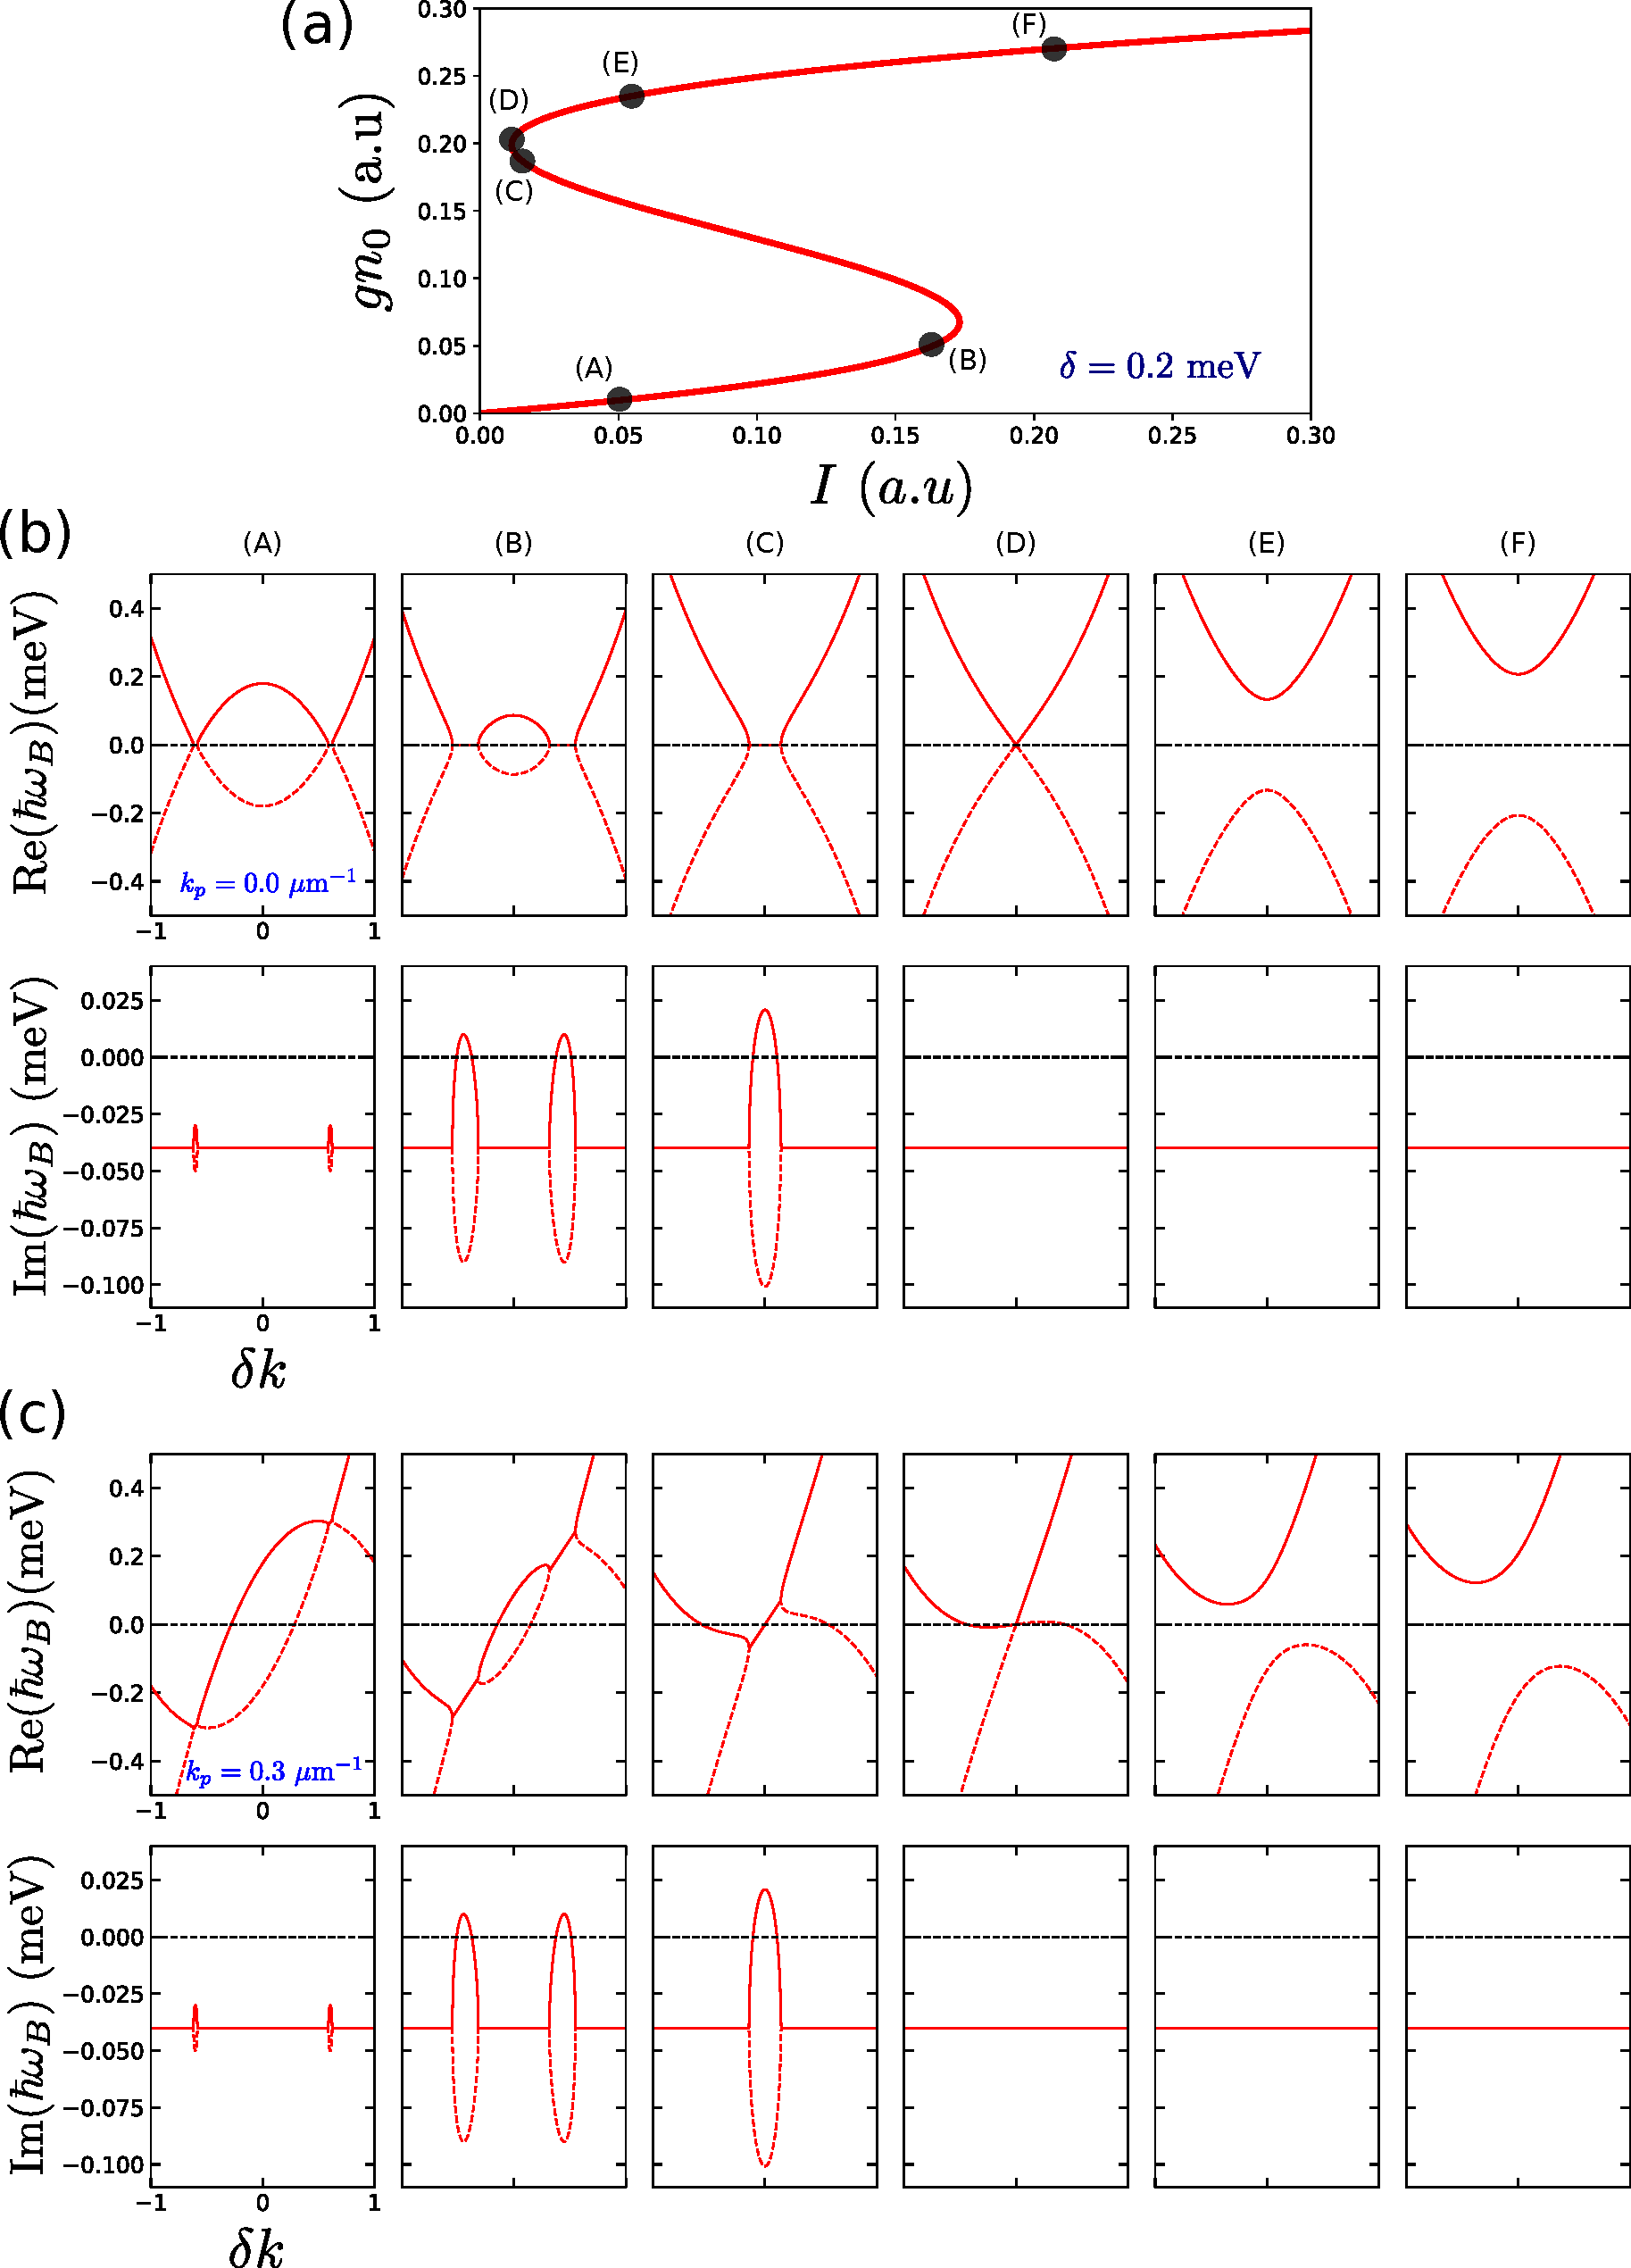
\includegraphics[width=1\textwidth]{chap_AG_theory/fig/bist_et_bogo.pdf}
\end{figure}
\addtocounter{figure}{-1}
\begin{figure} 
    \caption{\textbf{Analytical Bogoliubov dispersion relations.} (a) Bistability curve of the fluid density $n_0$ as a function of the pump intensity $I$, calculated from \autoref{eq:steady_state}, for a pump detuning $\hbar\delta$ = 0.2 meV. (b) Positive (solid red lines) and negative (dashed red lines) solutions of the Bogoliubov dispersion relation in the fluid reference frame, computed from \autoref{eq:bogo_lab_frame}, at the pump wavevector $\kbf_p$ = 0 (zero flow velocity), at the pump detuning $\delta(0)$ = 0.2 meV and for pump intensities indicated by the points A, ..., F in (a). Upper line: real part of the energy of elementary excitations. The black dotted line highlights the pump energy. Lower line: imaginary part of the energy of the elementary excitations. As long as it remains negative (below the black dashed line), the Bogoliubov solutions are dynamically stable. Note that near and all along the negative slope branch of the bistability, the modes are unstable, giving rise at the point B and C respectively to modulation instabilities (coupling of the positive solution with the negative solution at $\kvec \neq 0$) and Kerr instabilities (coupling of the positive and the negative solutions with the pump mode at $\kvec = 0$). At the other points A, D, E, F, the system losses fix the imaginary part at $-\gamlp/2$, stabilizing the fluid. (c) Same considerations as for (b) but for a pump wavevector $k_p$ = 0.5 $\mu$m$^{-1}$. The fluid speed of flow is no longer zero, leading to an asymmetrization of the Bogoliubov solutions. In both (a) and (b) cases, the linearization of the solutions at low-k, relating the generation of phonon-type elementary excitations, appears only at the turning point D. \textit{Adapted from} \cite{claude_phd}}
    \label{fig:bist_et_bogo}
\end{figure}

\bigskip 

\textbf{Linear spectrum.}
Let us first examine the most distinctive regime, which establishes a direct connection with conservative systems and was, in fact, the primary motivation for exploring this platform in the context of analog gravity experiments \cite{claude_high-resolution_2022}.
When the fluid operates at the turning point of the bistability (D) we demonstrated in the previous chapter that the detuning compensates the total interaction blueshift $\delta(0)=g_rn_r + gn_0$. 
Plugging this constraint in \autoref{eq:bogo_static} we obtain :

\begin{equation}
    \omega_B(k) = \pm \sqrt{\dfrac{\hbar k^2}{2\mlp} \left({\dfrac{\hbar k^2}{2\mlp}} + g n_0 \right)}.
\end{equation}

We introduce the healing length $\xi=\sqrt{\hbar^2/mgn_0}$ which is the characteristic length scale of the system below which the collective description of the fluid breaks down and microscopic effects
must be taken into account. The spectrum exhibits two trends depending whether $k$ is smaller or larger than $1/\xi$ as shown on the (D) plot of \autoref{fig:bist_et_bogo} \textbf{b)}. At low wavevector $k \ll 1/ \xi$ the spectrum is linear, for the normal branch we have :

\begin{equation}
    \re(\omega^+_B(k)) \sim c_s\abs{k}
\end{equation}
where $c_s = \sqrt{\hbar g n_0/\mlp}$ is the speed of sound in the fluid. For the ghost branch, represented by the red dashed line $c_s$ is be replaced by $-c_s$. At this operating point the driving laser is forcing the system exactly at its proper energy or said differently it is perfeclty resonant with 
microcavity. In this regime, the long range interactions are dominated by collective deformations of the fluid --phonons-- that propagate with the same group velocity $\partial\omega/\partial k =c_s$ regardless their wavevector. 
The idea of having --in the low wavevector limit -- a fixed velocity at all frequencies reminds the light cone with the difference that the sound velocity is not the same in all the reference frames.
The linearity is a typical feature of quantum fluids and gives rise to spectacular collective behavior such as superfluidity \cite{Amo_fluidlightexp_2009} as well as topological protection of quantized vortices and dark solitons \cite{maitre_thesis}.
The bogoliuvov spectrum was reported in several experiments \cite{utsunomiya_observation_2008,stepanov_dispersion_2019} with different experimental methods while the linearity has been measured with 
an unprecedented resolution in the group \cite{claude_high-resolution_2022}. The latter experiment was performed with a spectroscopy method recently developped \cite{claude_prb} that we will describe and use in the next chapter.

\bigskip

In the high wavevector limit, $k \gg 1/\xi $, we recover the standard parabolic dispersion blueshifted by the interaction.

\begin{equation}
    \re\left(\ombog^+(k)\right) \sim \dfrac{\hbar k^2}{2\mlp} + g n.
\end{equation}

It's worth noticing that at even higher wavevector the parabolic approximation is not valid anymore and the full LP dispersion must be plugged in the Bogoliubov matrix. In this case one would observe that the Bogoliubov spectrum is flattened
by the exciton line at large wavevector \cite{I_frerot_PRX_2023}.

\bigskip

\textbf{Massive excitations regime.} If the system is brought further along the upper bistability branch ie if $gn_0+g_rn_r>\delta(0)$ a gap opens in the spectrum and linearity is lost as it can be seen 
in plots (E) and (F). A limited development of the spectrum around $k=0$ gives the parabolic approximation:
\begin{equation}
    \re\left(\ombog^+(k)\right) \sim \omega^+_B(0) + \dfrac{\hbar k^2}{2\mlp}\dfrac{\left(2g n_0 + g_r n_r - \delta(0)\right)}{\sqrt{\left(2g n_0 + g_r n_r - \delta(0)\right)^2 - (g n_0)^2}}.
\end{equation}
This enables to provide the Bogoliubov modes with an effective mass :
\begin{equation}
    m_{\mathrm{det}}= \mlp\dfrac{\sqrt{\left(2g n_0 + g_r n_r - \delta(0)\right)^2 - (g n_0)^2}}{\left(2g n_0 + g_r n_r - \delta(0)\right)}.
\end{equation}
Note that in the limit $gn_0+g_rn_r\to \delta(0)$, the system recovers the massless scenario described earlier. 
The emergence of a gap in the spectrum can be understood as a form of "rigidity" in the fluid's phase, since introducing a phase fluctuation into the system requires a minimum energy.

\bigskip

In both the previous regimes, the terms in the square root of \autoref{eq:bogo_static} remain positive at all wavevectors meaning the imaginary part of 
full dispersion never deviates from $\gamma/2$ as shown in the subpanels of \autoref{fig:bist_et_bogo} \textbf{b)} ensuring the stability of the system.

\bigskip

\textbf{Low density regime.} Conversely, when the sytem is operating on the lower branch of the hysteresis loop, the amount of interaction is not sufficient to 
compensates for the detuning. Equivalently, it means that for some value of the wavevector the term in the square root of \autoref{eq:bogo_static} becomes negative
giving rise to additionnal contribution to the imaginary part of the spectrum. Note that it does not necessarily mean that the system is unstable. Indeed, an instability 
requires that the overall imaginary part of $\omega^{\pm}_B$ is positive. At very low density like in (A), the inherent losses of the system 
are sufficient to dump the instability and the imaginary part remains negative at all $k$. If the pump strength is ramped up near the lower branch turning point (B) 
the imaginary part of the spectrum might become positive at some wavevector and makes the system unstable. Note that the point at which this happens depends on the experimental
parameters. Finally, the point (C), located between the two branches, has an imaginary part that is highly positive at low wavevectors. This is the reason why this branch of excitation
is often referred as unstable and can not be observed. 


\bigskip 

The discussion above also holds for the case of a moving fluid provided we set our description in the comoving frame and replace $k$ by $\delta k=k-k_p$ in \autoref{eq:bogo_static}.

\subsubsection{Moving polaritons at finite $k_p$}
In this section we consider again a fluid in motion at $\kbf_p\neq0$ that we describe in the lab frame. In terms of regime of collective excitations, the phenomenology is similar to the one
described above and the discussion can be carried out in the same way. The only difference is that the dispersion relation is now centered around the fluid wavevector $\kbf_p$ and "tilted" by the Doppler effect. Consequently, the Bogoliubov spectrum graphically 
looses an axis of symmetry which is a graphical manifestation that $\Lbog$ no longer respects the symmetry of \autoref{eq:symmetry_bog}.
Again we set $\delta(k_p)=0.2 \mathrm{meV}$ and we plot the dispersion relation for the same operating points as in the static case, the results are presented in the subpanels of \autoref{fig:bist_et_bogo} \textbf{c)}. Note that the spectra are displayed as functions 
of the wavevector in the fluid frame since \autoref{eq:bogo_lab_frame} mathematically depends only on $\delta k$ enabling to compare the spectra in the two reference frames.

\begin{figure}[!htbp]
    \centering
    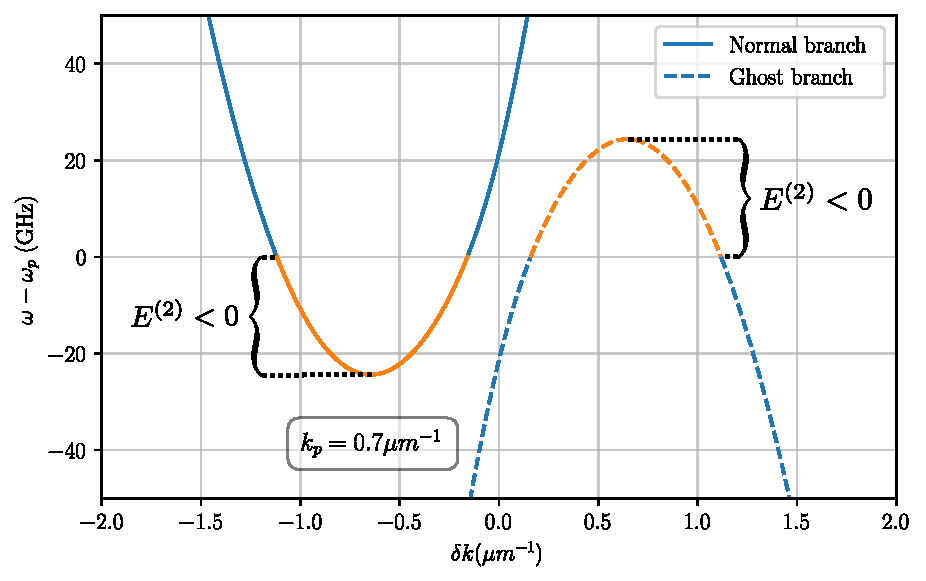
\includegraphics[width=\textwidth]{chap_AG_theory/fig/bogo_gap_supersonic_dispersion.pdf}
    \caption{Bogoliubov spectrum for a fluid in motion at $k_p=0.7 \mathrm{\mu m^{-1}}$ and $\delta(k_p)=0.2 \ \mathrm{meV}$. The dashed line represents the ghost branch ie the negative norm branch while the solid line
    represents the normal branch ie the positive norm branch. The blue color represents the positive energy modes while the orange represent the negative energy modes resulting from the 
    product of a norm and a frequency with opposite signs.}
    \label{fig:gapped_supersonic}
\end{figure}

In the linear case $gn_0+g_rn_r=\delta(k_p)$, the low wavevector slope is modified by the fluid velocity :
\begin{equation}
    \begin{aligned}
    \re\left(\ombog^+(\delta k)\right)& \sim (c_s + \vbf_0)\abs{\delta k} \ \ \mathrm{for} \ \delta k > 0 \\
    \re\left(\ombog^+(\delta k)\right)& \sim (c_s - \vbf_0)\abs{\delta k} \ \ \mathrm{for} \ \delta k < 0
    \end{aligned}
\end{equation}
From this, one can see that when the fluid is supersonic $\vbf_0>c_s$ as in plot (D) some modes of the normal branch --the positive norm modes-- are pulled down to the negative frequency domain. Symmetrically, some ghost branch modes --the negative norm modes-- are pulled up to the positive frequency domain.
In both cases, the excitations carry negative energy as explained in \autoref{subsub:bogo_energy}. In this regime, superfluidity is lost and any defect in the fluid flow 
can create excitations \cite{Amo_fluidlightexp_2009}. If the pump intensity is increased further like in (E) and (F), a gap opens again in the spectrum, the excitations are massive while
the negative energy modes may disappear due to the gap opening. However, it does not mean that the possibility to create excitations with negative energy 
is lost as soon as the spectrum is no longer linear. Indeed, increasing further the pump velocity can lead to situations where the spectrum is massive but still has negative energy modes.
A typical example of this case is presented in \autoref{fig:gapped_supersonic}, where the pump wavevector was set to $k_p=0.7 \mathrm{\mu m^{-1}}$ and the other parameters stayed the same. 
A gap is present but the Doppler effect is strong enough to excite negative energy modes on both branches which are represented by the orange lines. Unlike the linear case, it is not possible to define 
a sound velocity for the low wavevector excitations. Consequently, the critical velocity to exceed for the apperance of negative energy modes does not match the velocity $\sqrt{\hbar g n_0/\mlp}$ that we still refer to as the sound velocity
by analogy with linear case. Moreover, since the velocity affects the dispersion itself through the detuning $\delta(k_p)$, the usual procedure of applying the Landau criterion---where the energy of excitations is modified solely through a Doppler shift $\omega_B(k) \to \omega_B'(k) + v_0 k$---is no longer valid. By that, we mean that changing the pump wavevctor while keeping all the other parameters equals (the pump power and frequency) will affect the interaction energy 
since the bistability loop is modified through the detuning. In this case, the spectrum itself is inherently altered by the fluid motion, meaning that the flow velocity does not simply act as a shift parameter but fundamentally changes the nature of the excitations.
 As a result, the criterion to observe negative energy waves must be modified to account for this direct dependence. In practice, the knowledge of an analytical 
 expression for the critical velocity is not necessary and knowing that there exist one is sufficient as we will see in the experimental section.
 




\bigskip



It is now clear that depending on its velocity and parameters the fluid can exhibit a rich variety of collective excitations. Let us summarize what we reviewed  so far in this chapter.
\begin{tcolorbox}[infernoSummary]
    \begin{itemize}
        \item The polariton fluid exhibits a rich variety of collective excitations depending on the pump intensity and detuning through the bistability curve. The different 
        modes are characterized by their norm and frequency.
        \item There exist a peculiar operating point at which the spectrum is linear allowing for the definition of a sound velocity $c_s=\sqrt{\hbar g n_0/\mlp}$.
        \item The spectrum can also be massive if the system is pumped further along the high density branch and the effective mass depend on the detuning and the pump intensity.
        \item In the low density regime, the spectrum can become unstable and exhibit a positive imaginary part. 
        \item Putting the fluid in motion can lead to the appereance of negative energy modes. The critical velocity for this to happen is a complex function of the detuning and the interactions. It does not 
         match the speed of sound $c_s$ as soon as the system does not operate at the turning point of the hysteresis loop.
    \end{itemize}
    \end{tcolorbox}


In particular, if we restrict ourselves to high density regime where, inherent losses appart, the Bogoliubov dispersion remains real, the fluid can be either subcritical --all the modes carry positive energy-- or supercritical --some modes carry negative energy.
This discussion on the different collective excitation regimes paves the way to already understand how Hawking radiation can be observed in a polariton fluid. Indeed, creating 
an interface between a subcritical and a supercitical region will mix positive and negative energy modes just as a gravitationnal event horizon would. Then, 
 showing that it can leads to paired correlated emission from vacuum will require to quantize the modes as we will see in the next section.

\section{Hawking radiation in a transcritical fluid}
 


\subsection{Inhomogeneous pumping}
We consider a driving pump defined as follow :

\begin{equation}
    F_p(r,t) = \left\{
        \begin{array}{ll}
            F_ue^{i(k_ux-\omega_p t)} & \mbox{if } \ x<x_h \\
            F_de^{i(k_dx-\omega_p t)} & \mbox{if} \ x>x_h
        \end{array}
    \right.
\end{equation}
where $x_h$ is an arbitrary position that will define the interface bewteen the two regions. The wavevectors are chosen so that $0<k_u<k_d$ and $k_d$ is sufficiently high to create a supercritical flow. The fluid is 
flowing toward the $x>0$ direction and the label $"u"$ and $"d"$ refer respectively to "upstream" and "downstream" region of the fluid with respect to the interface. We want to study Hawking emission of propagating modes so we set 
the laser frequency in order to ensure bistability in both regions namely $\delta(k_u),\ \delta(k_d)>\sqrt{3}\gamlp/2$, and the pump amplitudes $F_u$ and $F_d$ in such a way that the fluids operate on the high density branch of their 
respective hysteresis cycle. Note that the pump is two dimensionnal but only depends on $x$. As we will justify it in the experimental section, the sample is in some extent also translationally invariant in the $y$ direction. Henceforth, we restrict our description to an effective 1D model.
Solving the GPE far from the interface gives two homogeneous regions with different asymptotic velocities $v_u=\hbar k_u/\mlp$ and $v_d=\hbar k_d/\mlp$, and different densities $n_u$ and $n_d$. We also 
account for fluctuations around each of these solutions the same way we did in the previous section which gives the asymptotic wavefunctions :

\begin{equation}
    \psi(x,t) = \left\{
        \begin{array}{ll}
            (\sqrt{n_u}+\dpsi_u)e^{i(k_ux-\omega_p t)} & \mbox{if } \ x \ll x_h \\
            (\sqrt{n_d}+\dpsi_d)e^{i(k_dx-\omega_p t)} & \mbox{if} \ x \gg x_h.
        \end{array}
    \right.
\end{equation}
While continuity conditions at $x_h$ makes the definition of the wavefunction near the interface unclear for now.
Typical density and velocity profiles are shown in \autoref{fig:velocity_and_density}. For the sake of clarity, the speed of sound rather than the density is plotted allowing direct comparison with 
the fluid velocity. We remind nonetheless that the previous section made clear that the relevant velocity to cross generally differs from $c_s$.

\begin{figure}[t!]
    \centering
    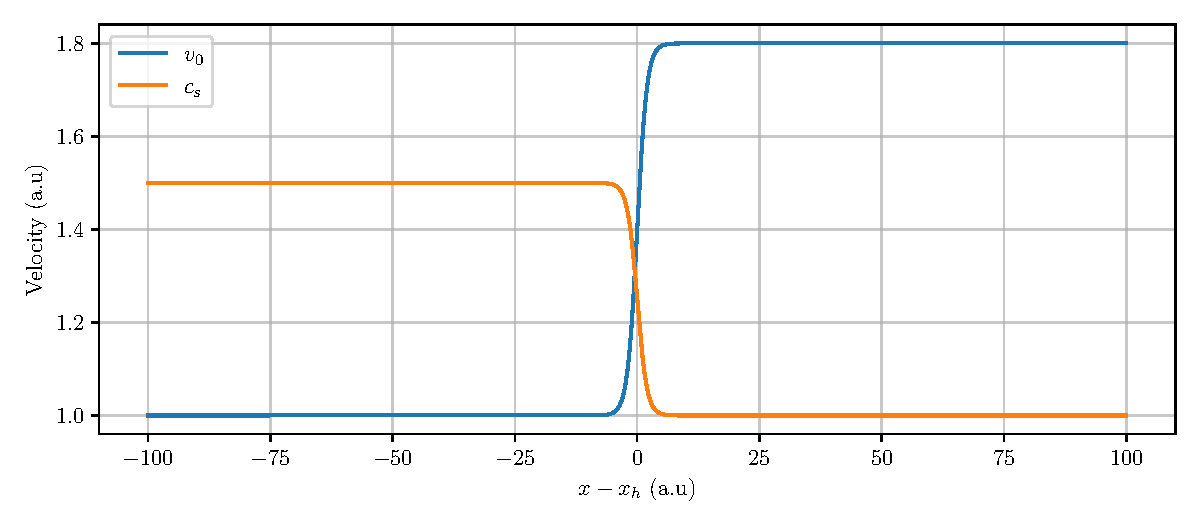
\includegraphics[width=1\textwidth]{chap_AG_theory/fig/typical_velocity.pdf}
    \caption{\textbf{Typical fluid and sound velocity profiles of a transcritical flow.} The blue line represents the fluid velocity $v_0(x)$ while the orange line represents the sound velocity $c_s(x)$.}
    \label{fig:velocity_and_density}
\end{figure}
\bigskip

We wish to solve the scattering problem for the Bogoliubov modes at the interface ie determine how a perturbation impinging on the analog horizon is scattered. In each homogeneous region, fluctuations are plane wave oscilating at $\omega$ of the form :
\begin{equation}
    \begin{pmatrix}
        u_k(x) \\
        v_k(x)
    \end{pmatrix} = \begin{pmatrix}
        U_k^u  \\
        V_k^u 
    \end{pmatrix}e^{i(k+k_{u,d})x}.
\end{equation}
The wavevector $k$ and frequency $\omega$ satisfy the Bogoliubov dispersion relation $\omega=\omega_B(k)$ that we remind here :

\begin{equation}
    \omega_B(k)=v_{u,d}k\pm\sqrt{\left(\dfrac{\hbar k^2}{2\mlp}-\delta(k_{u,d})+ g_rn_r +2g n_0\right)^2 - \left(g n_0\right)^2}-\dfrac{i\gamma}{2} 
    \label{eq:bogo_lab_frame_both_regions}
\end{equation}
where $v_{u,d}=\hbar k_{u,d}/\mlp$ are the fluid velocities in the upstream and downstream regions. The corresponding dispersions are plotted in \autoref{fig:bogo_up_and_down}. We see that, in the subcritical region ($x<x_h$), positive- and negative-norm modes are still found exclusively at positive and negative frequency, respectively.
However, in the supercritical region ($x>x_h$), some positive-norm modes are dragged to negative frequencies (and reciprocally for negative-norm modes) by the Doppler effect.

\bigskip


Since there is redundancy of the information with respect to the zero frequency line let us fix $\omega>0$ and look for the wavevectors $k$ satisfying $\omega=\omega_B(k)$ in each region.
\begin{figure}
    \centering
    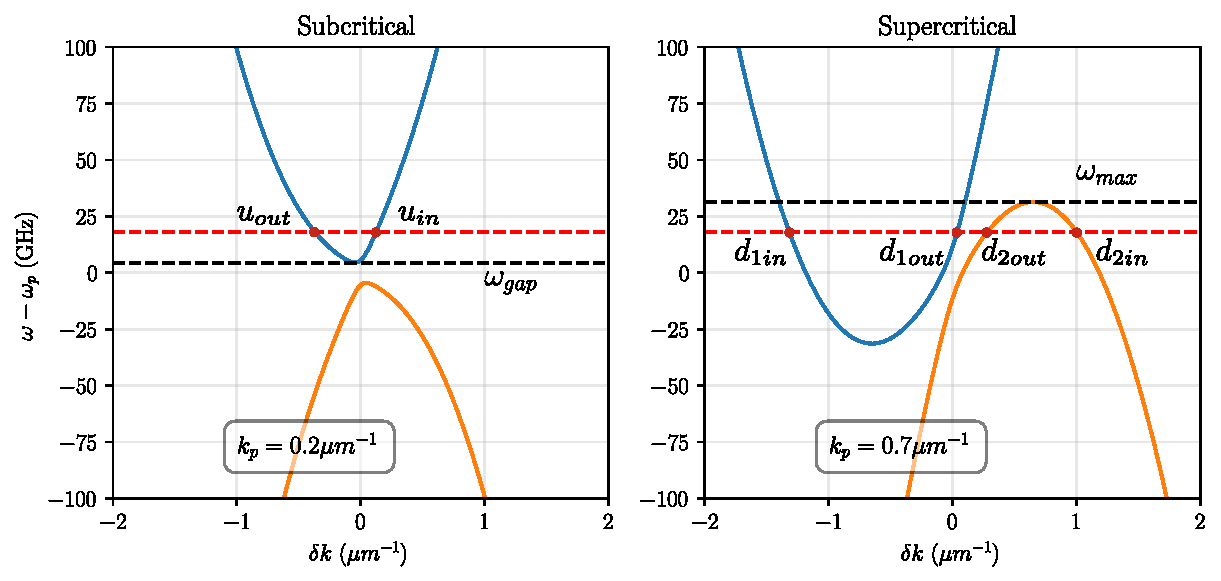
\includegraphics[width=1\textwidth]{chap_AG_theory/fig/bogo_gap_dispersion.pdf}
    \caption{\textbf{Bogoliubov spectrum in the upstream and downstream regions.} The Bogoliubov spectrum in the asymptotic upstream region \textbf{(a)} and downstream region \textbf{(b)} of the fluid, calculated from \autoref{eq:bogo_lab_frame} with $\delta(0)=30$ (GHz), $k_u= \SI{0.2}{\per \micro \meter}$ and
    $k_d=\SI{0.7}{\per\micro\meter}$.}
    \label{fig:bogo_up_and_down}
\end{figure}

\bigskip

\textbf{Subcritical region.} In the upstream region $x<xh$, for any $\omega>\omega_{gap}$ where $\omega{gap}=\min{\omega^+_B(k)}$ there always exist two real solutions corresponding to positive norm modes as visible on the left panel of \autoref{fig:bogo_up_and_down}. Depending
on the sign of their group velocity $v_g=\partial\omega/\partial k$, we label the solution $'out'$ if it propagates away from the interface and $'in'$ if it goes toward the interface. 
Taking the square of \autoref{eq:bogo_lab_frame_both_regions} the problem can be cast under a real coefficient polynomial equation of degree 4 in $k$. As a consequence,
there exist two additional complex conjugate solutions. Depending on the sign of their imaginary part, they are either exponentially growing or decaying. Note that for $0<\omega<\omega_{gap}$, the four solutions are non propagating with imaginary wavevectors.

\bigskip


\textbf{Supercritical region.} In the downstream region $x>x_h$, the situation is different and requires a different analysis. If $\omega>\omega_{max}$ where $\omega_{max}=\max{\omega^-_B(k)}$, the situation is the same as in the upstream 
region. There exists two propagating solutions $d_{1in}$ and $d_{1out}$ lying on the normal branch with opposite group velocity as well as two non propagating modes. When $\omega<\omega_{max}$, in addition to the positive norm solution, the Doppler shift pulls two negative norm solutions $d_{2in}$ and $d_{2out}$ inherited from $\omega=\omega^-_B(k)$

So far, the modes we have identified are defined locally, in the sense that a Bogoliubov plane wave that is a solution to the equations of motion in the upstream region is not a solution in the downstream region, and vice versa. Let us now
see how we can construct global modes (GM) that are defined everywhere in the system and satisfy the equations of motion in both regions.
\bigskip

\textbf{Scattering solutions-\textit{in} global modes}
A general function to describe the fluctuations at $\omega$ is obtained by the linear combination of all the possible propagating solutions :
\begin{equation}
    \begin{pmatrix}
        u_k(x) \\
        v_k(x)
    \end{pmatrix}_{u,d} = \left(\sum_{i\in \mathrm{in}}\betin_i e^{ik^{in}_ix}\begin{pmatrix}
        U_{k^\mathrm{in}_i}  \\
        V_{k^\mathrm{in}_i}
    \end{pmatrix}+\sum_{i\in \mathrm{out}}\betout_i e^{ik^{out}_ix}\begin{pmatrix}
        U_{k^\mathrm{out}_i}  \\
        V_{k^\mathrm{out}_i}
    \end{pmatrix}\right)_{u,d}
\end{equation}
From this expression we can form the so-called scattering solutions. Such a solution reflects how a given local mode impinging on the interface is scattered into the other channels.
For instance, for the case of an incoming mode from the upstream region, the scattering solution is a piece-wise function given by :


\begin{align}
    \begin{pmatrix}
        u_k(x) \\
        v_k(x)
    \end{pmatrix}_{u} &=\betin_ue^{{ik_u^{{\mathrm{in}}x}}}\begin{pmatrix}
        U_{k^\mathrm{in}_{u}} \\
        V_{k^\mathrm{in}_{u}}
    \end{pmatrix}
    +
    \betout_u e^{ik_u^{{\mathrm{out}}x}}\begin{pmatrix}
        U_{k^\mathrm{out}_{u}} \\
        V_{k^\mathrm{out}_{u}}
    \end{pmatrix} \ \mathrm{for} \ x\leq x_h \\
    \begin{pmatrix}
        u_k(x) \\
        v_k(x)
    \end{pmatrix}_{d} &= \betout_{d2} e^{ik^{\mathrm{out}}_{d2}x}
    \begin{pmatrix}
        U_{k^\mathrm{out}_{d2}} \\
        V_{k^\mathrm{out}_{d2}}
    \end{pmatrix} + \betout_{d1} e^{ik^{\mathrm{out}}_{d1}x}
    \begin{pmatrix}
        U_{k^\mathrm{out}_{d1}} \\
        V_{k^\mathrm{out}_{d1}} 
    \end{pmatrix} \ \mathrm{for} \ x\geq x_h.
\end{align}

A given solution and its derivative has to be continuous in space which imposes matching conditions at the interface. This condition will fix the coefficients $\beta_i^{in}$ and $\beta_i^{out}$ that can be interpreted as reflexion and transmission coefficients of the incoming wave at the interface. 
These modes are defined over the entire space and satisfy the equations of motion everywhere. From the three $in$ local modes--$u_{in}$, $d_{1in}$ and $d_{2in}$--in the $\omega_{gap}<\omega<\omega_{max}$ regime it is possible to construct three global scattering solutions by following the same reasoning. At a given frequency $\omega$ one can verify that these solutions are orthonormal with respect to the Bogoliubov inner product :
\begin{equation}
    \begin{aligned}
    \bra{\dpsi^\mathrm{in}_i(\omega)}\ket{\dpsi^\mathrm{in}_j(\omega')}_B &= \int \mathrm{d}x  \ [u^*_{i,\omega}(x)u_{j,\omega'}(x)-v^*_{i,\omega}(x)v_{j,\omega'}(x)]  \\
    &= \mathrm{sign}(\bra{\psi^\mathrm{in}_i}\ket{\psi^\mathrm{in}_i}_B)\delta_{ij}\delta(\omega-\omega'),
    \end{aligned}
    \label{eq:in_global_modes}
\end{equation} 
where $i,j \in \{u_{in},d_{1in},d_{2in}\}$ and $\mathrm{sign}$ is the sign function. 
As defined, the $in$ global modes (GM) form a basis of the Bogoliubov problem valid at any $x$ in the system.

\bigskip

\textbf{Outgoing global modes.} It is also possible to define the global solution of an outgoing wave. Take the outgoing mode $d_{1out}$ in the downstream region : in the scattering picture it originates from 
 the transmission of an ingoing upstream mode $u_{in}$ and the reflexion of the two ingoing downstream modes $d_{2in}$ and $d_{1in}$. Doing this procedure in the $\omega_{gap}<\omega<\omega_{max}$ range, the three $out$ modes
define three outgoing GM. Just as the $in$ solutions, the $out$ ones form an orthonormal basis of the solution space.

Since we found two basis describing the same set it is possible to express the $out$ modes in terms of the $in$ modes. 
Each three $out$ modes are linear combination of the three $in$ modes which define the so called $3\times3$ scattering matrix $S(\omega)$ :

\begin{equation}
    \begin{pmatrix}
        \betout_{u}(\omega) \\
        \betout_{d1}(\omega) \\
        \betout_{d2}(\omega)
        \end{pmatrix} =
    S(\omega)\begin{pmatrix}
        \betin_{u}(\omega) \\
        \betin_{d1}(\omega) \\
        \betin_{d2}(\omega)
    \end{pmatrix}.
    \label{eq:scattering_matrix}
\end{equation}
Note that in $\omega>\omega_{max}$ case the $d_{2out}$ mode is not present and the scattering matrix should be $2\times2$. However, to keep 
the notation the same everywhere, we also take into account the evanescent modes and allow some coefficient to be zero in the scattering matrix.

Since the orthonormal structure of the Bogoliubov modes was built with the modified norm $\bra{\cdot}\ket{\cdot}_B$ it implies
that $S$ is unitary for the corresponding extented metric $\nu$ :

\begin{equation}
    S^\dagger(\omega)\eta S(\omega) = \eta.
    \label{eq:unitarity}
\end{equation}
where $\eta=\mathrm{diag}(1,1,-1)$. The unitary condition ensures energy conservation even in the presence of negative energy modes.  Indeed, the $-1$ sign in the third diagonal term account for norm conversion and originate from the scattering of positive norm modes into negative norm modes.
The square modulus of a given coefficient $\abs{S_{ij}}^2$ gives the probability of reflexion or transmission of the mode $i$ into the mode $j$.

To make this point clear, let us consider the example of the scattering of an incoming mode $u_{in}$ with energy $\hbar\omega$ in the upstream region. 
There is a probability $\abs{S_{uu}}^2$ that the mode gets reflected in $u_{out}$ and a probability $\abs{S_{d1u}}^2$ that it gets transmitted into $d_{1out}$ : both these modes have the same energy. The remaining term $\abs{S_{u2}}^2$ is the probability of transmission into a negative norm mode $d_{2out}$ whith the opposite energy $-\hbar\omega$
The unitary condition \autoref{eq:unitarity} ensures that the total energy is conserved $1=\abs{S_{uu}}^2+\abs{S_{d1u}}^2-\abs{S_{d2u}}^2$. Note that a complete 
derivation of the scattering matrix in an ideal step like case as well as a numerical study case was done for conservative systems in \cite{Recati_acousticHR_2009} and \cite{fabbri_steplike_2011} respectively.


It is interesting to stress that the asymptotic classification of modes as $in$ or $out$ mirrors the procedure used in the study of quantum fields in black hole spacetimes, where a causal, time-oriented interpretation is adopted: in modes represent incoming configurations in the remote past, while out modes correspond to outgoing configurations in the distant future.
 This structure forms the basis of the Bogoliubov transformation formalism, which relates the two bases and captures the mixing between positive and negative frequency components that underlies processes such as particle production.
\subsection{Modes quantization}
\label{subsec:quantization}
So far, we described the fluctuations of the order parameter as classical fields. This approach
shows that the Bogoliubov modes can exist in the system as solutions to the equations of motion. The scattering matrix
 tells us how an incoming wavepacket is scattered at the interface \cite{Recati_acousticHR_2009}.
Yet, our classical description requires an external perturbation to inject a given mode. Hence, it does not
predict what would happen with highly non-classical state as an input, like the vacuum state. To achieve this, we need to quantize the modes.

\bigskip
\textbf{Quadratic Hamiltonian.} The first step is to write the field operator : 
\begin{equation}
    \hat{\psi}(x,t)= \psi_0(x,t)\hat{a}_{\psi_0}+\hat{\dpsi}(x)
\end{equation}
where $\hat{a}_{\psi_0}$ is the operator that annihilates a polariton in the mean field state and $\hat{\dpsi}(x)$ is the fluctuation operator that 
annihilates a fluctuation particle. Plugging this ansatz into the GPE in its second quantization form \ref{eq:pol_non_linear_hamiltonian} and going to first order in the fluctuations, one
finds that the hamiltonian has a quadratic form in the fluctuation operator. As a consequence, the Heisenberg
equations of motion for the Bogoliubov operator are linear in the fluctuations \cite{castin_bose-einstein_2001}. This property is of great importance.
Indeed, it allows using a very simple quantization procedure. The fully quantum decomposition of the 
fluctuation operator is obtained from its classical counterpart ~\ref{eq:general_solution_for_fluctuations_classical} by promoting the coefficients $b_k$ to bosonic operators. A $u$ coefficient is associated to an annihilation operator while a $v$ coefficient is associated to a creation operator.
 Under this prescription--whose validity is rigorously justified in \cite{castin_low-temperature_1998}--the classical fluctuations field becomes :

\begin{equation}
    \delta\hat{\psi}(x,t) =\sum_{k}\left[u_k(x)\bk e^{-i\omega_k t}+ v^*_k(x)\bkdag e^{i\omega_k t}\right]
\end{equation}
with the commutation relation 
\begin{equation}
    \norm{\phi_i}_B\norm{\phi_j}_B[\hat{b}_i, \hat{b}_j^\dagger]  = \norm{\phi_i}_B\delta_{ij}
\end{equation}
which is the usual bosonic commutation relation for positive norm modes while for negative norm modes the annihilation operator and the creation operator are exchanged. To encode this property in a convenient way in the notation we rewrite the fluctuation field in a such a way that for negative norm modes an annihilation operator
is associated to the $v$ component as :

\begin{equation}
    \delta\hat{\psi}(x,t) =\sum_{k\in S_+}\left[u_k(x)\bk e^{-i\omega_k t}+ v^*_k(x)\bkdag e^{i\omega_k t}\right] + \sum_{k\in S_-}\left[u_k(x)\bkdag e^{-i\omega_k t}+ v^*_k(x)\bk e^{i\omega_k t}\right]
    \label{eq:fluctuation_field_local_modes}
\end{equation}
This formulation has the advantage of making explicit that for negative norm modes the frequency $\omega_k$ is associated to annihilation operators reflecting the particle-hole symmetry :
the creation of a particle a yields the same contribution as the annihilation of a hole.



This procedure remains valid regardless the basis initially chosen and can especially be applied to the global modes exhibited earlier. The fully quantized fluctuations field can then be expressed in terms of $in$ global operators as \cite{Recati_acousticHR_2009}:

\begin{equation}
    \hat{\dpsi}(x,t) = \int \mathrm{d}\omega\sum_{j\in \{u_{in},d_{1in}\} }[\ha_j(\omega)u_{j,\omega}(x)+\hadag_j(\omega)v^*_{j,\omega}(x)] + \int \mathrm{d}\omega[\hadag_{d_2}(\omega)u_{d_2,\omega}(x)+\ha_{d_2}(\omega)v^*_{d_2,\omega}(x)]
    \label{eq:fluctuation_quantization}
\end{equation}
where the operator $\hat{a}_j(\omega)$ is the operator that annihilates a global $in$ mode in channel $j$ at frequency $\omega$. An equivalent
expression can be written for the $out$ global modes noted $\hb_i$. The two sets of operators are again related by the scattering matrix :

\begin{equation}
    \begin{pmatrix}
        \hat{b}_u(\omega) \\
        \hat{b}_{d1}(\omega) \\
        \hat{b}_{d2}^\dagger(\omega)
    \end{pmatrix}=S(\omega)\begin{pmatrix}
        \hat{a}_u(\omega) \\
        \hat{a}_{d1}(\omega) \\
        \hat{a}_{d2}^\dagger(\omega)    
    \end{pmatrix}
\end{equation}


Few comments can be done at this stage. First, since we deal with quadratic Hamiltonian, the matrix is exactly the same as that obtained in the classical case.
From an experimental point of view this property is a crucial asset. Indeed, it means one can reconstruct the full matrix and hence all its quantum 
properties by just solving the scattering problem for classical modes which are much easier to engineer than quantum state. Any quantum correlations between the modes are in fact encoded in the matrix coefficients 
under phase and amplitude values. Of course, solving the scattering problem
would only be a way to infer correlations between the modes but not to measure them. Still, it gives information about what you can expect from a given 
analog horizon.

\bigskip

Secondly, while the $in$ and $out$ operators describe the same physical system they generate two different Fock states and thus two distinct vacuum states $\ket{0_{\mathrm{in}}}$ and $\ket{0_{\mathrm{out}}}$. Indeed, the vacuum 
is ultimately defined by the Hamiltonian and thus of the operators used to describe the system.
This raises the question of whether a preferential basis can be found to provide an unequivocal description of the system. In fact, when a system does not exhibit time or space symmetries it is generally not the case \cite{qft_wald_chicago_1994}. In quantum field theory on curved spacetime, the Hamiltonian is typically time-dependent, which makes it difficult to define a unique set of operators and an unambiguous vacuum state. For instance, in the Unruh effect \cite{unruh_!notes_1976}, an accelerating observer detects thermal radiation whereas an inertial observer perceives the 'standard' vacuum. 
This ambiguity lies at the core of particle creation processes in general.

 This being said, the $in$ and $out$ basis remain, in the present case, wise choices to describe the system since they are natural basis to infer what can be measured in the lab.

\bigskip

Finally, we reminded at the beginning of this chapter that the wave equation describing the fluctuations on top of a moving polariton fluid could be casted under Klein-Gordon 
equation for a massive real scalar field in a curved spacetime. Treating the polariton fluid with the Bogoliubov theory showed that the formal equivalence with black hole equations
could be pushed one step further by the presence of a Bogoliubov transformation between the $in$ and $out$ basis induced by the scattering matrix.

To say this in one sentence : while being very different, these two systems have in common the presence of a horizon that mixes positive and negative energy modes. The polariton platform is then an interesting system to study quantum field theory predictions --initially made for gravitational event horizons-- through the universality of the underlying 
mathematical structure, a Bogoliubov transformation \cite{unruh_universality_2005,hangleiter_analogue_2022}. This universality allows to study a wide classe of "superradiant" phenomena \cite{brito_superradiance_2020_lectures} sharing the common feature of creating entanglement \cite{rot_supperradiance_delhom}.

\subsection{Spontaneous emission}

\label{subsec:spontaneous_emission}

Now that we have a fully quantized description of the system, expectation values of physical observables can be straightforwardly
computed by plugging the desired input quantum state and look how it is modified by the scattering matrix. Let us start with the most spectacular effect, that
Stephen Hawking demonstrated in his original work \cite{hawking_black_1972} : spontaneous emission of correlated pairs from vacuum.


We are interested in the expectation value of the outgoing mode that is radiated by the interface away from the supercritical region $\hat{b}_u$.
Its decomposition in terms of the $in$ modes is :

\begin{equation}
    \hat{b}_u = S_{uu}\hat{a}_u + S_{ud_1}\hat{a}_{d_1} + S_{ud_2}\hat{a}_{d_2}^\dagger.
\end{equation}
The corresponding number operator $\hat{N}_u^{out}=\hat{b}_u^\dagger\hat{b}_u$ then reads :
\begin{equation}
    \begin{aligned}
        \hat{N}_u^{out} = &\abs{S_{uu}}^2\hat{a}_u^\dagger\hat{a}_u + \abs{S_{ud_1}}^2\hat{a}_{d_1}^\dagger\hat{a}_{d_1} + \abs{S_{ud_2}}^2\hat{a}_{d_2}\hat{a}_{d_2}^\dagger \\ 
        + & S_{uu}^*S_{ud_1}\hat{a}_u^\dagger\hat{a}_{d_1}+ S_{uu}^*S_{ud_2}\hat{a}_u^\dagger\hat{a}_{d_2}^\dagger + S_{ud_1}^*S_{uu}\hat{a}_u^\dagger\hat{a}_{d_1}^\dagger  \\
        + & S_{ud_1}^*S_{ud_2}\hat{a}_{d_1}^\dagger\hat{a}_{d_2}^\dagger+ S_{ud_2}^*S_{uu}\hat{a}_{d_2}\hat{a}_u+ S_{ud_2}^*S_{ud_1}\hat{a}_{d_2}\hat{a}_{d_1}. 
    \end{aligned}
\end{equation}
Using the bosonic commutation relation for the negative norm term $\abs{S_{ud_2}}^2\hat{a}_{d_2}\hat{a}_{d_2}^\dagger=\abs{S_{ud_2}}^2(1+\hat{a}_{d_2}^\dagger\hat{a}_{d_2})$, the expectation
value of the number operator in the $in$ vacuum state $\ket{0_{in}}$ is :

\begin{equation}
    \bra{0_{in}}\hat{N}_u^{out}\ket{0_{in}} = \abs{S_{ud_2}}^2 
\end{equation}
In the $\omega \notin [\omega_{gap}, \omega_{max}]$ frequency range, the $d_2$ mode is not present and there is no emisssion. Conversely, when $\omega_{gap}<\omega<\omega_{max}$ 
the negative energy mode $d_2$ is present and yields a non zero emission from vacuum. This is the so-called Hawking effect. In fact,
 this radiation is correlated with all the other outgoing modes and one could even show tripartite entanglement among them \cite{isoard_quantum_2019}. Nonetheless, this is beyond the
 scope of this work and we will not go into the details of this calculation.

\bigskip

 \textbf{State of the art.} Usually in the litterature, correlations at the horizon 
 between the out mode are inferred by computing the two points density correlation function \cite{Recati_acousticHR_2009, nguyen_acoustic_2015} :

 \begin{equation}
    g^{(2)}(x,x')=\dfrac{\langle{\hat{\dpsi}}^\dagger(x)\hat{\dpsi}^\dagger(x')\hat{\dpsi}(x)\hat{\dpsi}(x')\rangle}{\langle \hat{\dpsi}^\dagger(x)\hat{\dpsi}(x)\rangle\langle \hat{\dpsi}^\dagger(x')\hat{\dpsi}(x')\rangle}
 \end{equation}
Several numerical studies have been performed first in conservative systems \cite{carusotto_numerical_2008} and then in polariton platforms \cite{nguyen_acoustic_2015,jacquet_quantum_2023} demonstrating that the horizon of a transcritical flow can indeed exhibit Hawking radiation signature in its density correlation map. 
A typical $g^(2)(x,x')$ map is shown in \autoref{fig:correlation_map}.

\begin{figure}[t!]
    \centering
    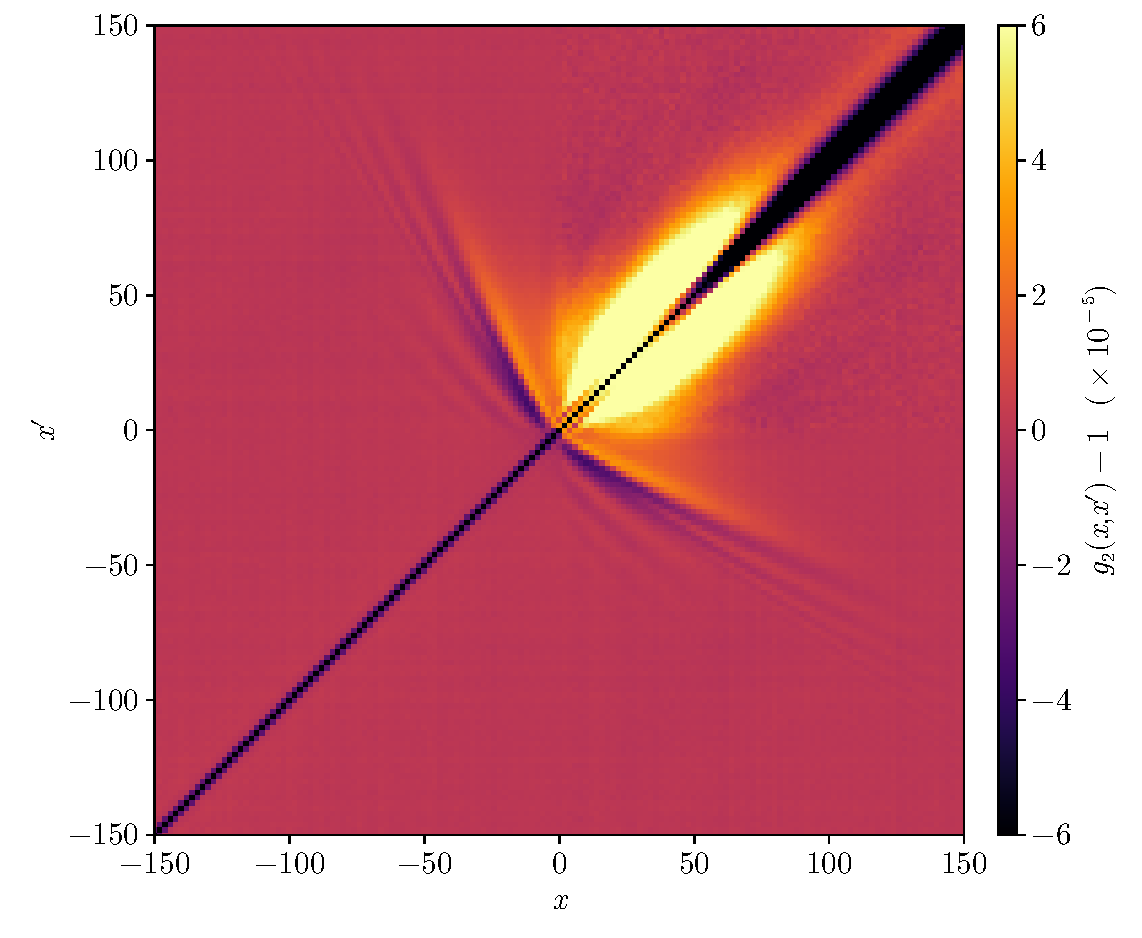
\includegraphics[width=1\textwidth]{chap_AG_theory/fig/g2_position.pdf}
    \caption{\textbf{Density correlation map.} Two points density correlation function $g^{(2)}(x,x')$ of a 1D transcritical polariton fluid. The correlation signal
    in the $x>0$ and $x'<0$ region (top-left panel) is the signature of the correlated Hawking emission at the horizon position $x=0$ .}
    \label{fig:correlation_map}
\end{figure}
An experimental measurement of this correlation map has already been performed in Bose Einstein Condensate of Rb atoms \cite{steinhauer_observation_2016}.
In this experiment, the same analog black hole is created 7400 times, each shot providing a realization of the density fluctuation map. The two points density correlation
function is then computed by taking the average of $\hat{\dpsi}^\dagger(x)\hat{\dpsi}^\dagger(x')\hat{\dpsi}(x)\hat{\dpsi}(x')$. In the case of a polariton fluid the density fluctuations map is harder to obtain due to 
the out of equilibrium nature of the system. Indeed, due to the finite lifetime of the polaritons $1/\gamma\sim \SI{10}{\pico \second}$, a single 
image of the fluid, even with the fastest camera, is already the result of many realizations of the fluctuations which hence average to zero. In the conservative case,
a given shot of the experiment limits the condensate time evolution on a finite time interval when the trap is released. Therefore, looking for spontaneous
emission in the polariton fluid is not a trivial task. However, the photonic nature of the polariton system allows to use many quantum optics techniques to look for correlation into other observables.
For instance, a homodyne detection should in principle be able to detect the horizon effect on the vacuum quadrature since it acts as a two mode squeezer \cite{agullo_symplectic_2022}. As a first approach one can look for a stimulated version of the experiment which, in the light of the previous section,
can be theoretically grasped by injecting a coherent state in the scattering problem. As we will see in \autoref{chap:stimulated_hawking}, the polariton platform is better suited
to look for signatures of Hawking radiation in momentum space and is closer to the theoretical proposal of \cite{fabbri_momentum_2018}.
\subsection{Stimulated emission}

Consider a coherent state input state $\ket{\alpha_{in}}$ in the upstream region, eigenstate of the annihilation operator $\hat{a}_u$ with eigenvalue $\alpha_u \in \mathbb{C}$. All the other 
input modes are left in the vacuum state which gives the overall input state :
\begin{equation}
    \ket{\alpha_{in}}=\ket{\alpha_u}\otimes\ket{0_{d_1}}\otimes\ket{0_{d_2}}.
\end{equation}
Using that $\hat{a}_u\ket{\alpha_{in}}=\alpha_u\ket{\alpha_{in}}$ the expectation value in this state is straightfrowardly computed as :
\begin{equation}
    \bra{\alpha_{in}}\hat{N}_u^{out}\ket{\alpha_{in}} = \abs{S_{uu}}^2\abs{\alpha_u}^2 + \abs{S_{ud_2}}^2\abs{\alpha_u}^2
    \label{eq:stimulated_expectation_value}
\end{equation}
The presence of a coherent input state gives rise to an additionnal term $\abs{S_{uu}}^2\abs{\alpha_u}^2$ which is the "classical" reflexion of the input mode at the interface.
To obtain a full scattering picture we also compute what is transferred in the other outgoig modes. The calculations are similar and we find :

\begin{equation}
    \bra{\alpha_{in}}\hat{N}_{d_1}^{out}\ket{\alpha_{in}} = \abs{S_{d_1u}}^2\abs{\alpha_u}^2 + \abs{S_{d_1d_2}}^2
    \label{eq:d1_stimulated_expectation_value}
\end{equation}
for the $d_1$ outgoing mode and 
\begin{equation}
    \bra{\alpha_{in}}\hat{N}_{d_2}^{out}\ket{\alpha_{in}} = \abs{S_{d_2u}}^2\abs{\alpha_u}^2 + \abs{S_{d_2d_2}}^2
    \label{eq:d2_stimulated_expectation_value}
\end{equation}
for the $d_2$ outgoing mode. This negative energy mode can be interpreted as the Hawking partner of the positive energy mode $u_{out}$.
If we assume that $\abs{\alpha_u}$ is large enough, the first term in each of the above equation dominates the second one which gives :

\begin{equation}
    \dfrac{\bra{\alpha_{in}}\hat{N}_i^{out}\ket{\alpha_{in}}}{\abs{\alpha_u}^2} \approx \abs{S_{i u}}^2 \ \mathrm{for} \ i\in\{u,d_1,d_2\}.
\end{equation}
This quantity is accessible in the lab since it amounts to measuring the classical reflexion and transmission coefficients of the interface when a
coherent state is sent toward the interface from the upstream region. Even though this feature is not triggered by quantum vacuum 
fluctuations it is still a manifestation of the Hawking effect. To understand this point one must compare the scenarios
whether $\omega$ is in $[\omega_{gap}, \omega_{max}]$ or not. In the latter case, energy conservation is simply $\abs{S_{uu}}^2\abs{\alpha_u}^2+\abs{S_{d_1u}}\abs{\alpha_u}^2=\abs{\alpha_u}^2$ and reflects that each of the output channels
carries a fraction of the incoming energy. While when $\omega \in [\omega_{gap}, \omega_{max}]$ the same condition reads $\abs{S_{uu}}^2\abs{\alpha_u}^2+\abs{S_{d_1u}}^2\abs{\alpha_u}^2-\abs{S_{d_2u}}^2\abs{\alpha_u}^2=\abs{\alpha_u}^2$ due to the negative energy mode.
This directly implies $\abs{S_{uu}}^2\abs{\alpha_u}^2+\abs{S_{d_1u}}^2\abs{\alpha_u}^2\geq \abs{\alpha_u}^2$ which means that the two positive energy channels
carry more energy than what was injected, the excess being compensated by the negative energy mode. This amplification means that the incoming 
coherent state extracted energy from the transcritical region by exciting a negative energy mode. This is the same 
argument that led to the prediction of rotational superradiance in black hole physics \cite{hawking_black_1972} as well as in classical electromagnetic systems \cite{zeldovich__1970}.

\section{Conclusion}

In this chapter, we have explored the theoretical framework underlying the observation of Hawking radiation in a polariton quantum fluid. Starting from the Gross-Pitaevskii equation, we derived the Bogoliubov spectrum of collective excitations, highlighting the rich variety of regimes depending on the fluid's density, velocity, and interaction strength. We demonstrated how the interplay between positive- and negative-energy modes leads to the possibility of particle creation at a transcritical interface, analogous to the Hawking effect in black hole physics.

The quantization of Bogoliubov modes revealed the fundamental role of the scattering matrix in describing the mixing of positive- and negative-norm modes at the horizon. This mixing not only enables spontaneous emission from vacuum but also provides a framework to study stimulated emission, where coherent input states amplify the Hawking-like radiation. Importantly, we showed that the amplification of outgoing modes is driven by the presence of negative-energy modes.

These results establish a theoretical foundation for the experimental investigation of analog Hawking radiation in polariton systems. By leveraging the properties of polariton fluids, such as their out-of-equilibrium nature and tunable parameters, this platform offers a promising avenue to probe fundamental aspects of quantum field theory in curved spacetime. In the next chapter, we will focus on the experimental implementation of these concepts and the challenges associated with observing Hawking radiation in practice.